Os resultados obtidos englobam a prototipação das telas da aplicação mobile, aplicação web em Node.js responsivo, os Diagramas de UML e de Redes, a Modelagem Lógica, Conceitual e comandos do Banco de Dados, do Modelo de Negócios Canvas.

\subparagraph*{\textbf{Prototipação do Figma}}

Na Figura 1, demonstra a tela inicial, onde o usuário é direcionado para a tela de login/cadastro para poder ser utilizado.

\begin{figure}[!htb]
\centering
\SetCaptionWidth{\ifbool{@LayoutA}{0.7}{0.72}\linewidth}
\caption{Tela Inicial}%
\label{fig:tela-inicial}
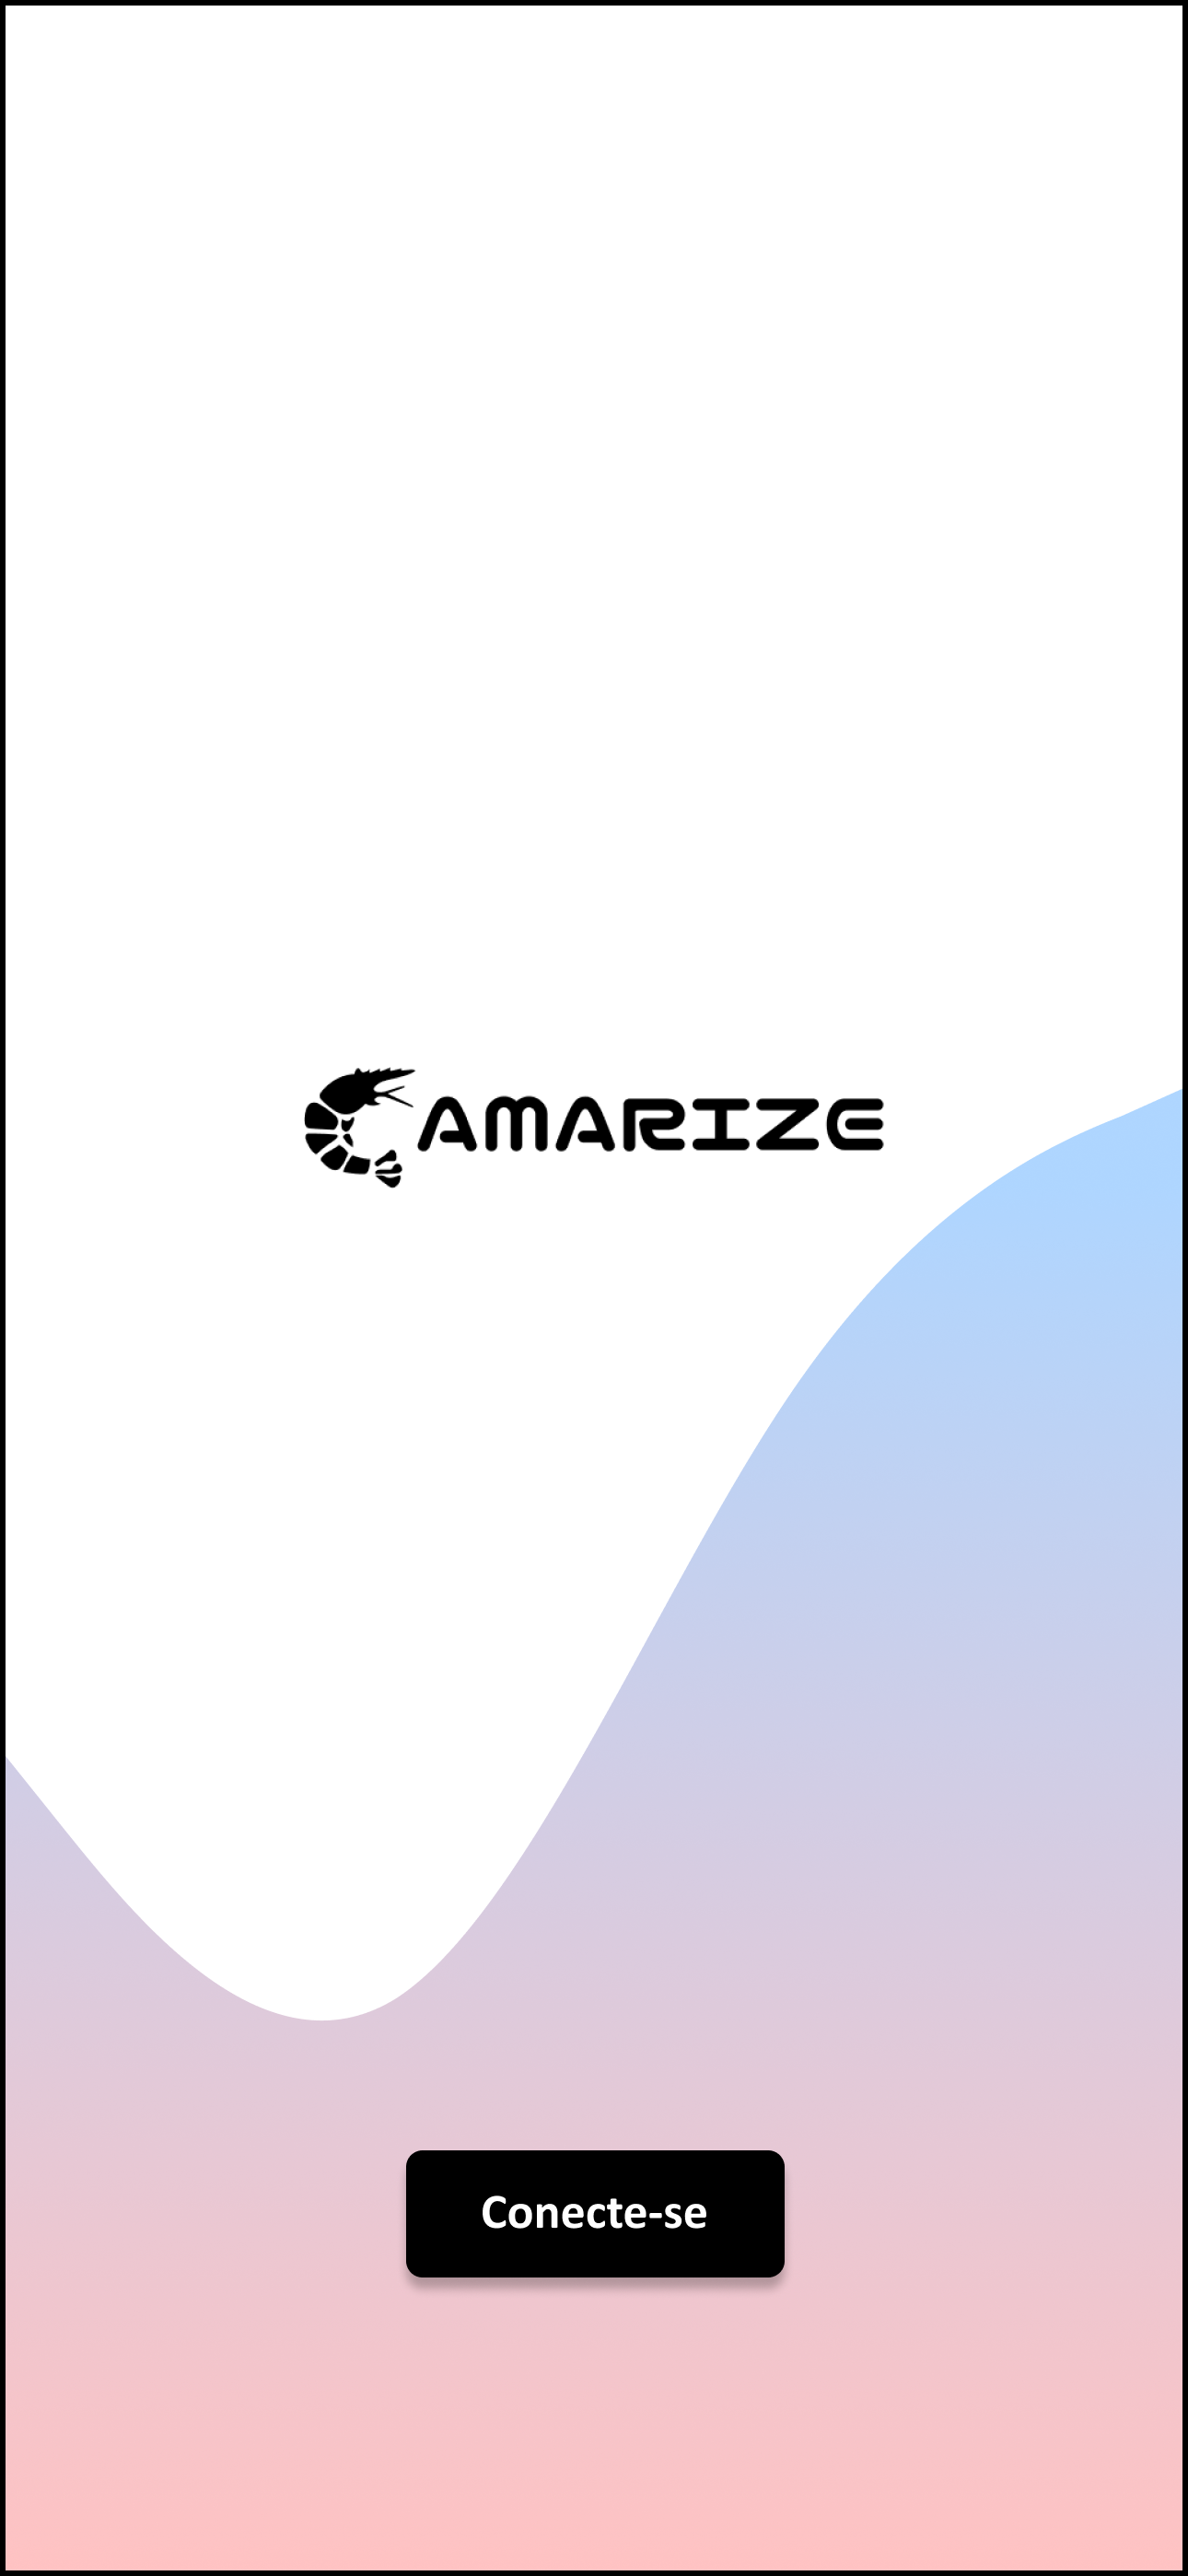
\includegraphics[width = 0.4\textwidth]{Imagem/Tela_Inicial.png}
\SourceOrNote{Autoria Própria, 2024}
\end{figure}

\newpage

Na Figura 2, é demonstrada a tela principal que mostra os tanques que o usuário registra. Em cada tanque, é possível observar um botão. Esse botão é utilizado para a escolha manual ou automático da alimentação dos camarões. Nos tanques, é possível realizar a edição dos cadastros de cada tanque. 

\begin{figure}[!htb]
\centering
\SetCaptionWidth{\ifbool{@LayoutA}{0.7}{0.72}\linewidth}
\caption{Tela Principal}%
\label{fig:tela-principal}
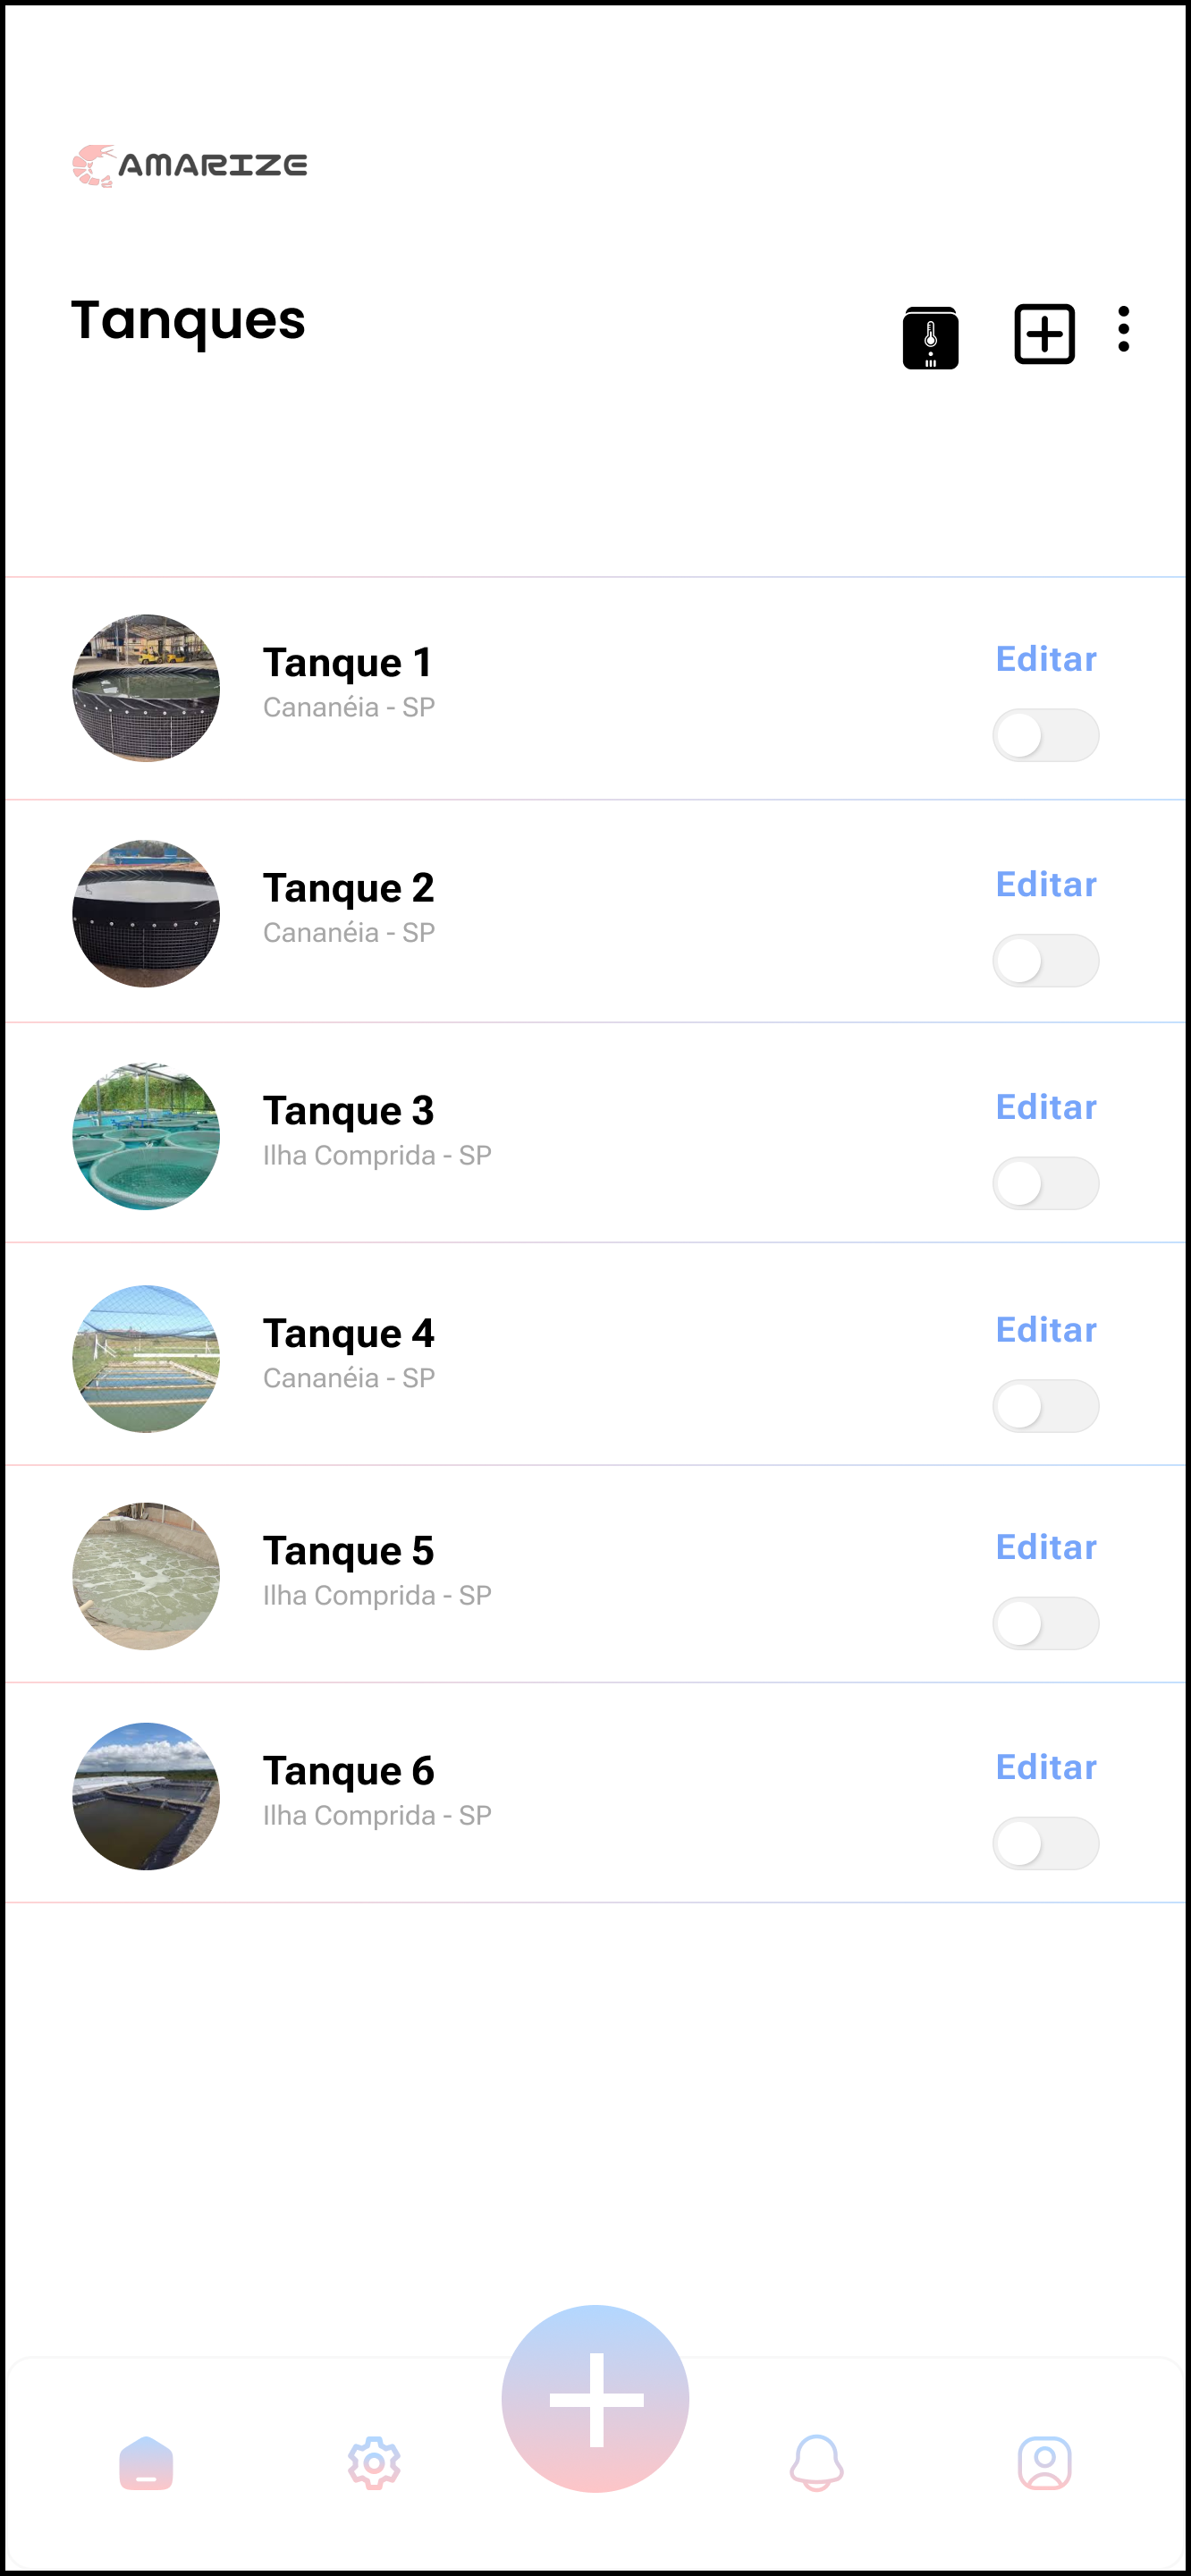
\includegraphics[width = 0.5\textwidth]{Imagem/Lista_Tanques.png}
\SourceOrNote{Autoria Própria, 2024}
\end{figure}

\newpage

Na Figura 3, é representada a tela de dashboard, esta tela pode ser visualizada após selecionar um tanque para verificar informações. Nesta tela, é possível verificar a temperatura do cativeiro, o pH, a amônia e dentre outras informações como camarões. É possível verificar um gráfico com registro de temperatura e pH de datas recentes.

\begin{figure}[!htb]
\centering
\SetCaptionWidth{\ifbool{@LayoutA}{0.7}{0.72}\linewidth}
\caption{Dashboard}%
\label{fig:tela-dashboard}
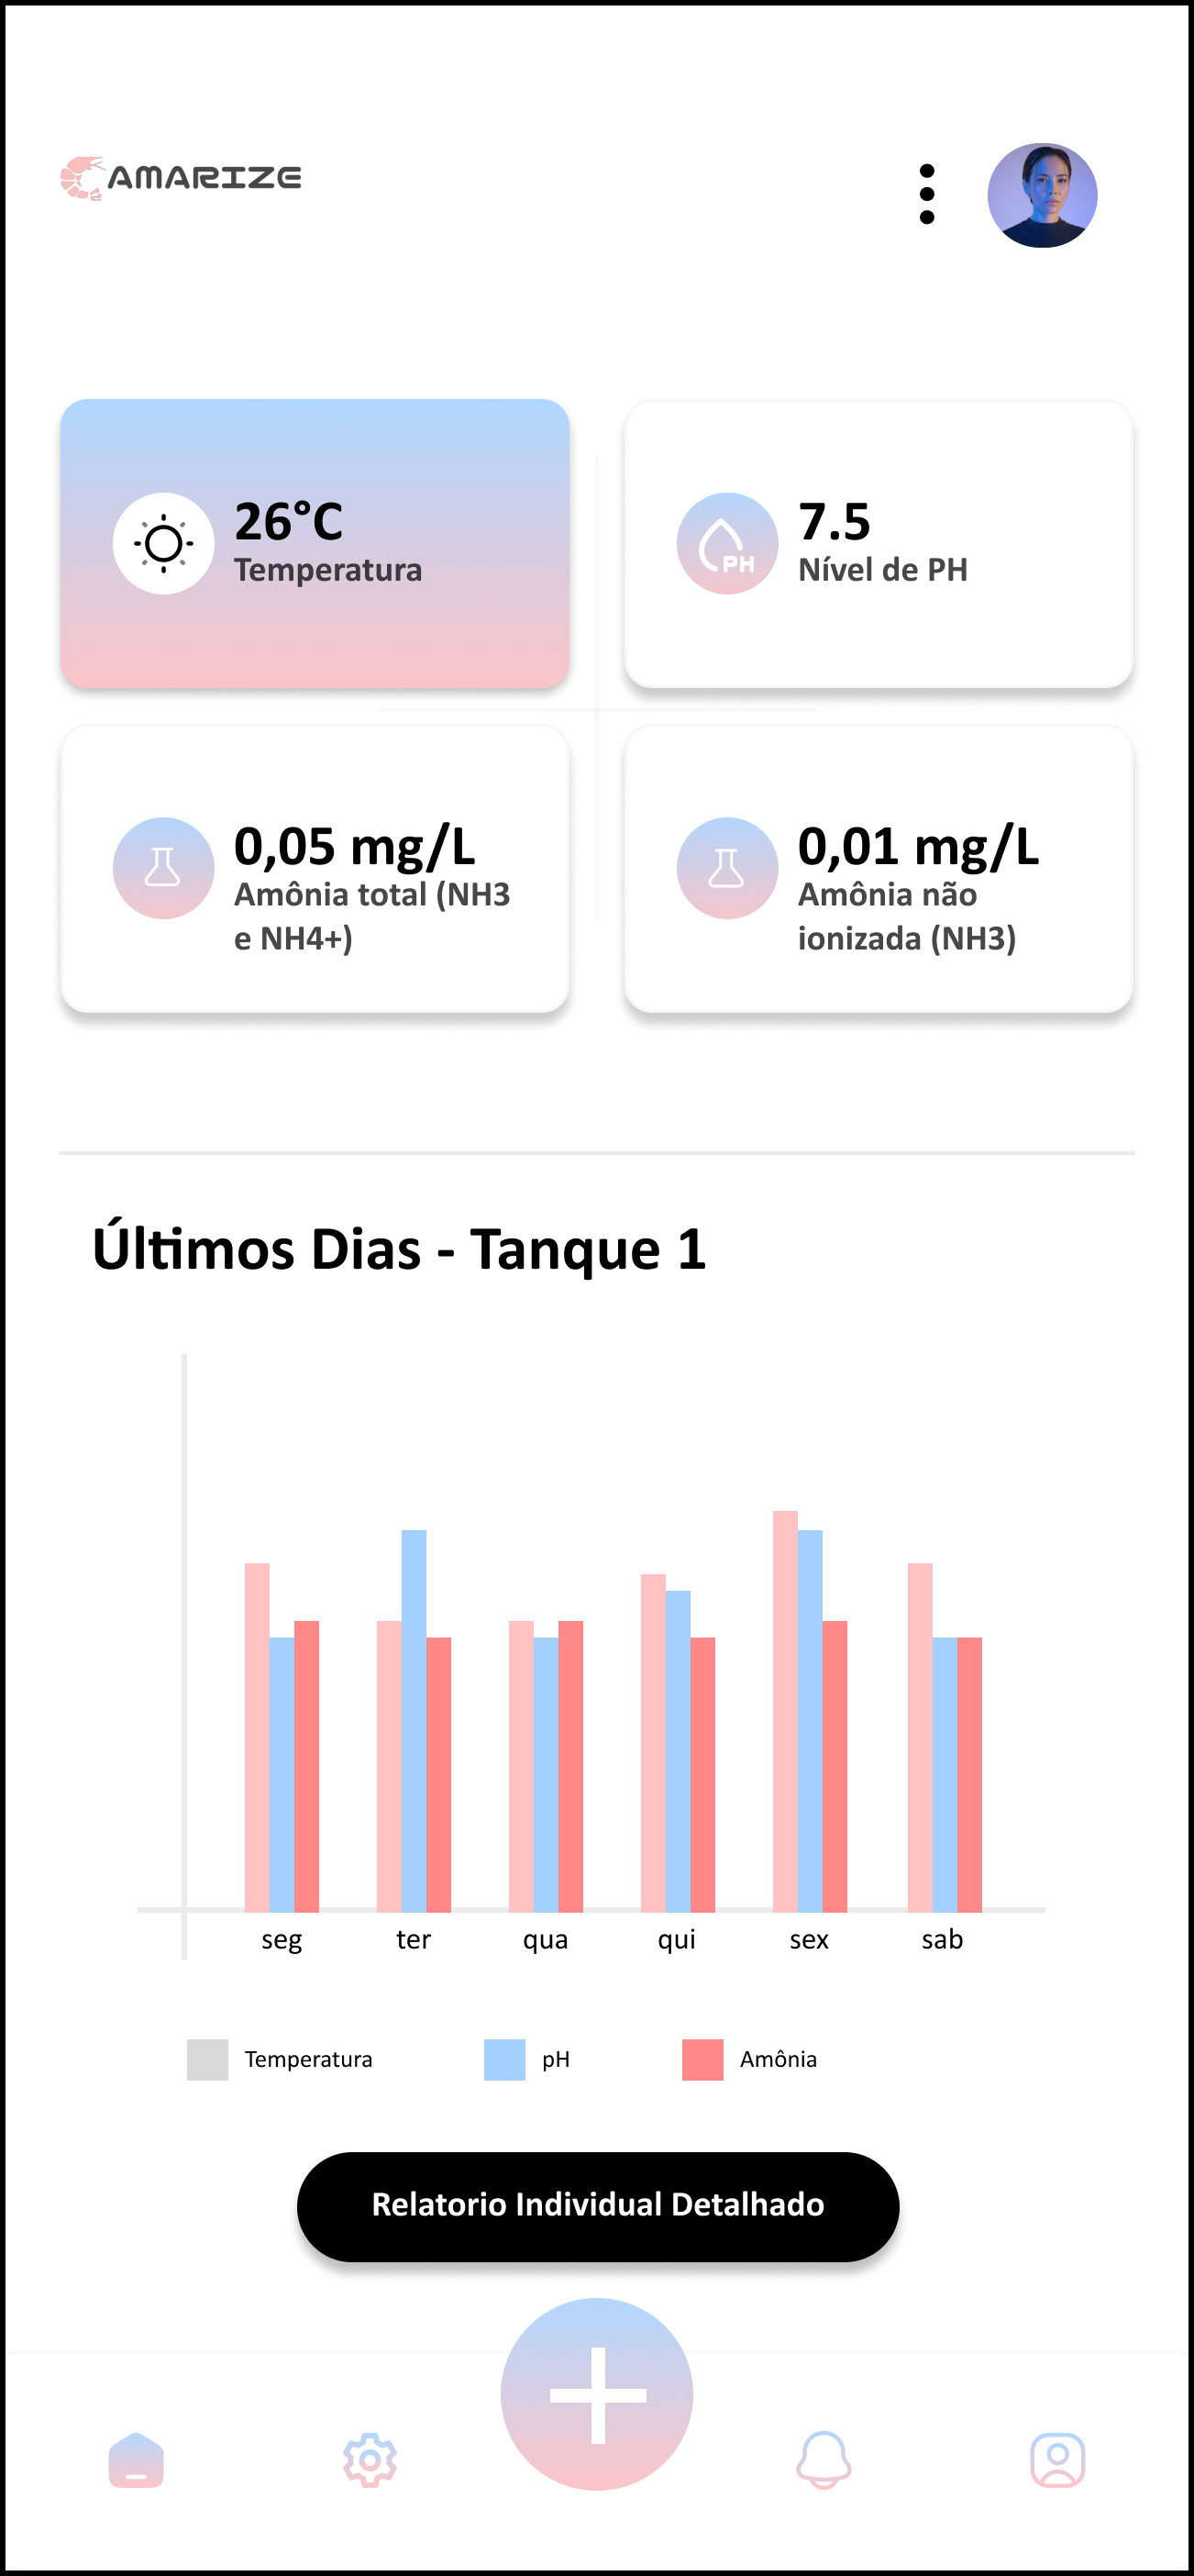
\includegraphics[width = 0.5\textwidth]{Imagem/Dashboard.png}
\SourceOrNote{Autoria Própria, 2024}
\end{figure}

\newpage

Na Figura 4, é representada a tela de equipamentos presentes em cada tanque, sendo possível editar as informações presentes e excluir.

\begin{figure}[!htb]
    \centering
    \SetCaptionWidth{\ifbool{@LayoutA}{0.7}{0.72}\linewidth}
    \caption{Equipamentos}%
    \label{fig:sistema}
    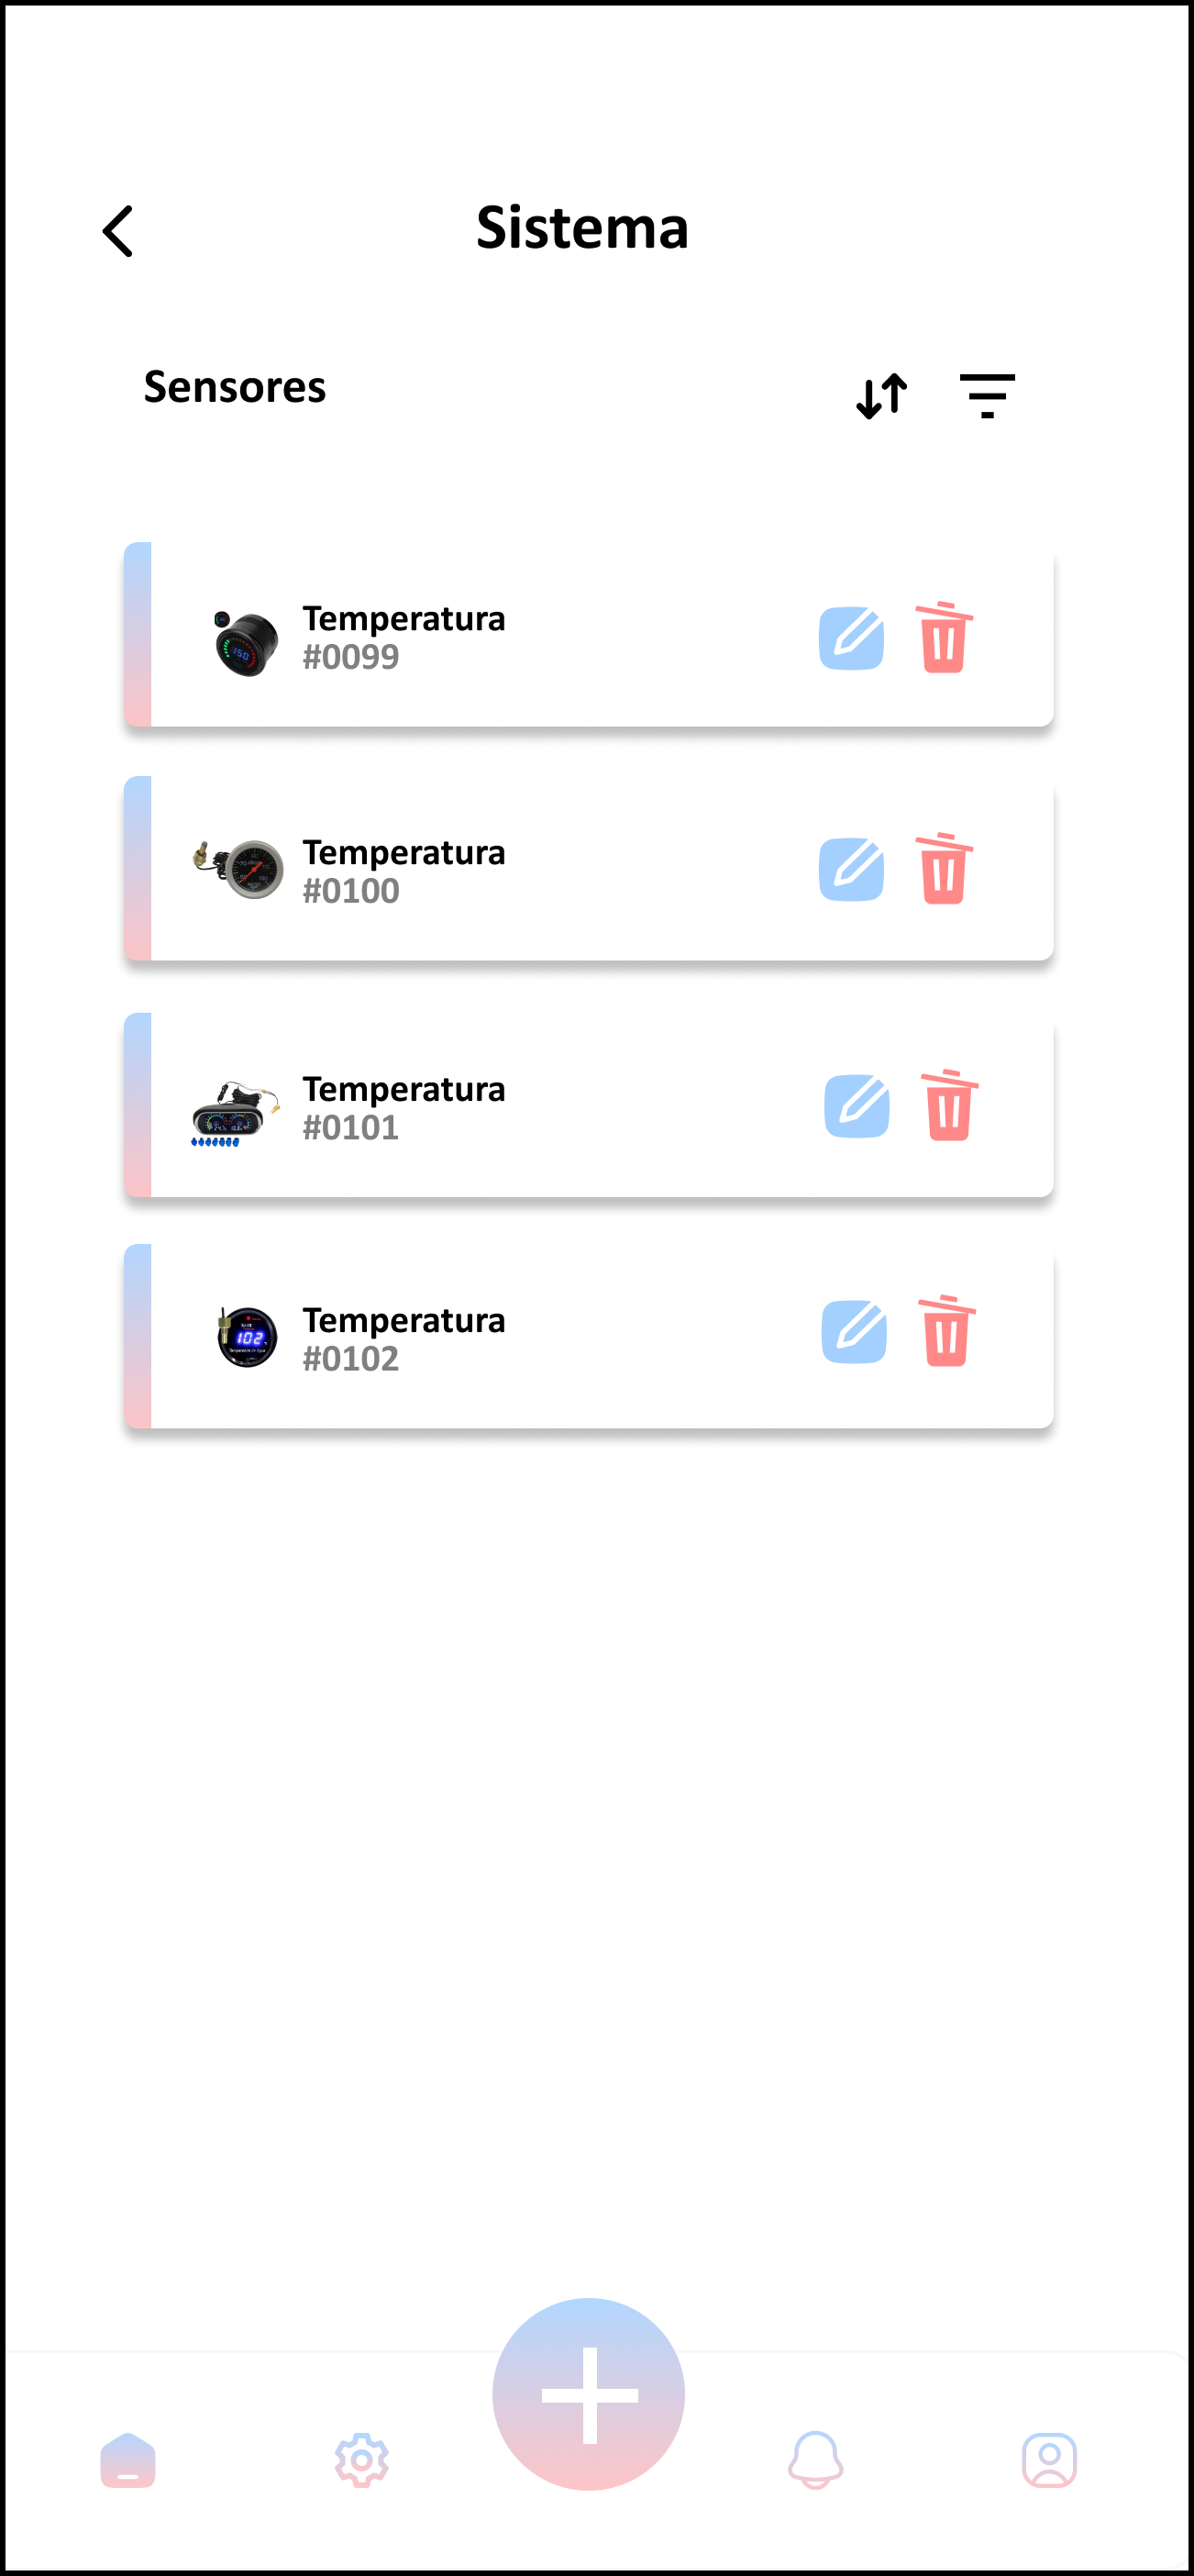
\includegraphics[width = 0.5\textwidth]{Imagem/Sistema.png}
    \SourceOrNote{Autoria Própria, 2024}
\end{figure}

\newpage

Na Figura 5, demonstra a tela de cadastro de sensor, onde é possível inserir o tipo de sensor, podendo ser sensor de temperatura, amônia e pH e uma foto para identificação do mesmo.

\begin{figure}[!htb]
    \centering
    \SetCaptionWidth{\ifbool{@LayoutA}{0.7}{0.72}\linewidth}
    \caption{Itens}%
    \label{fig:sensor}
    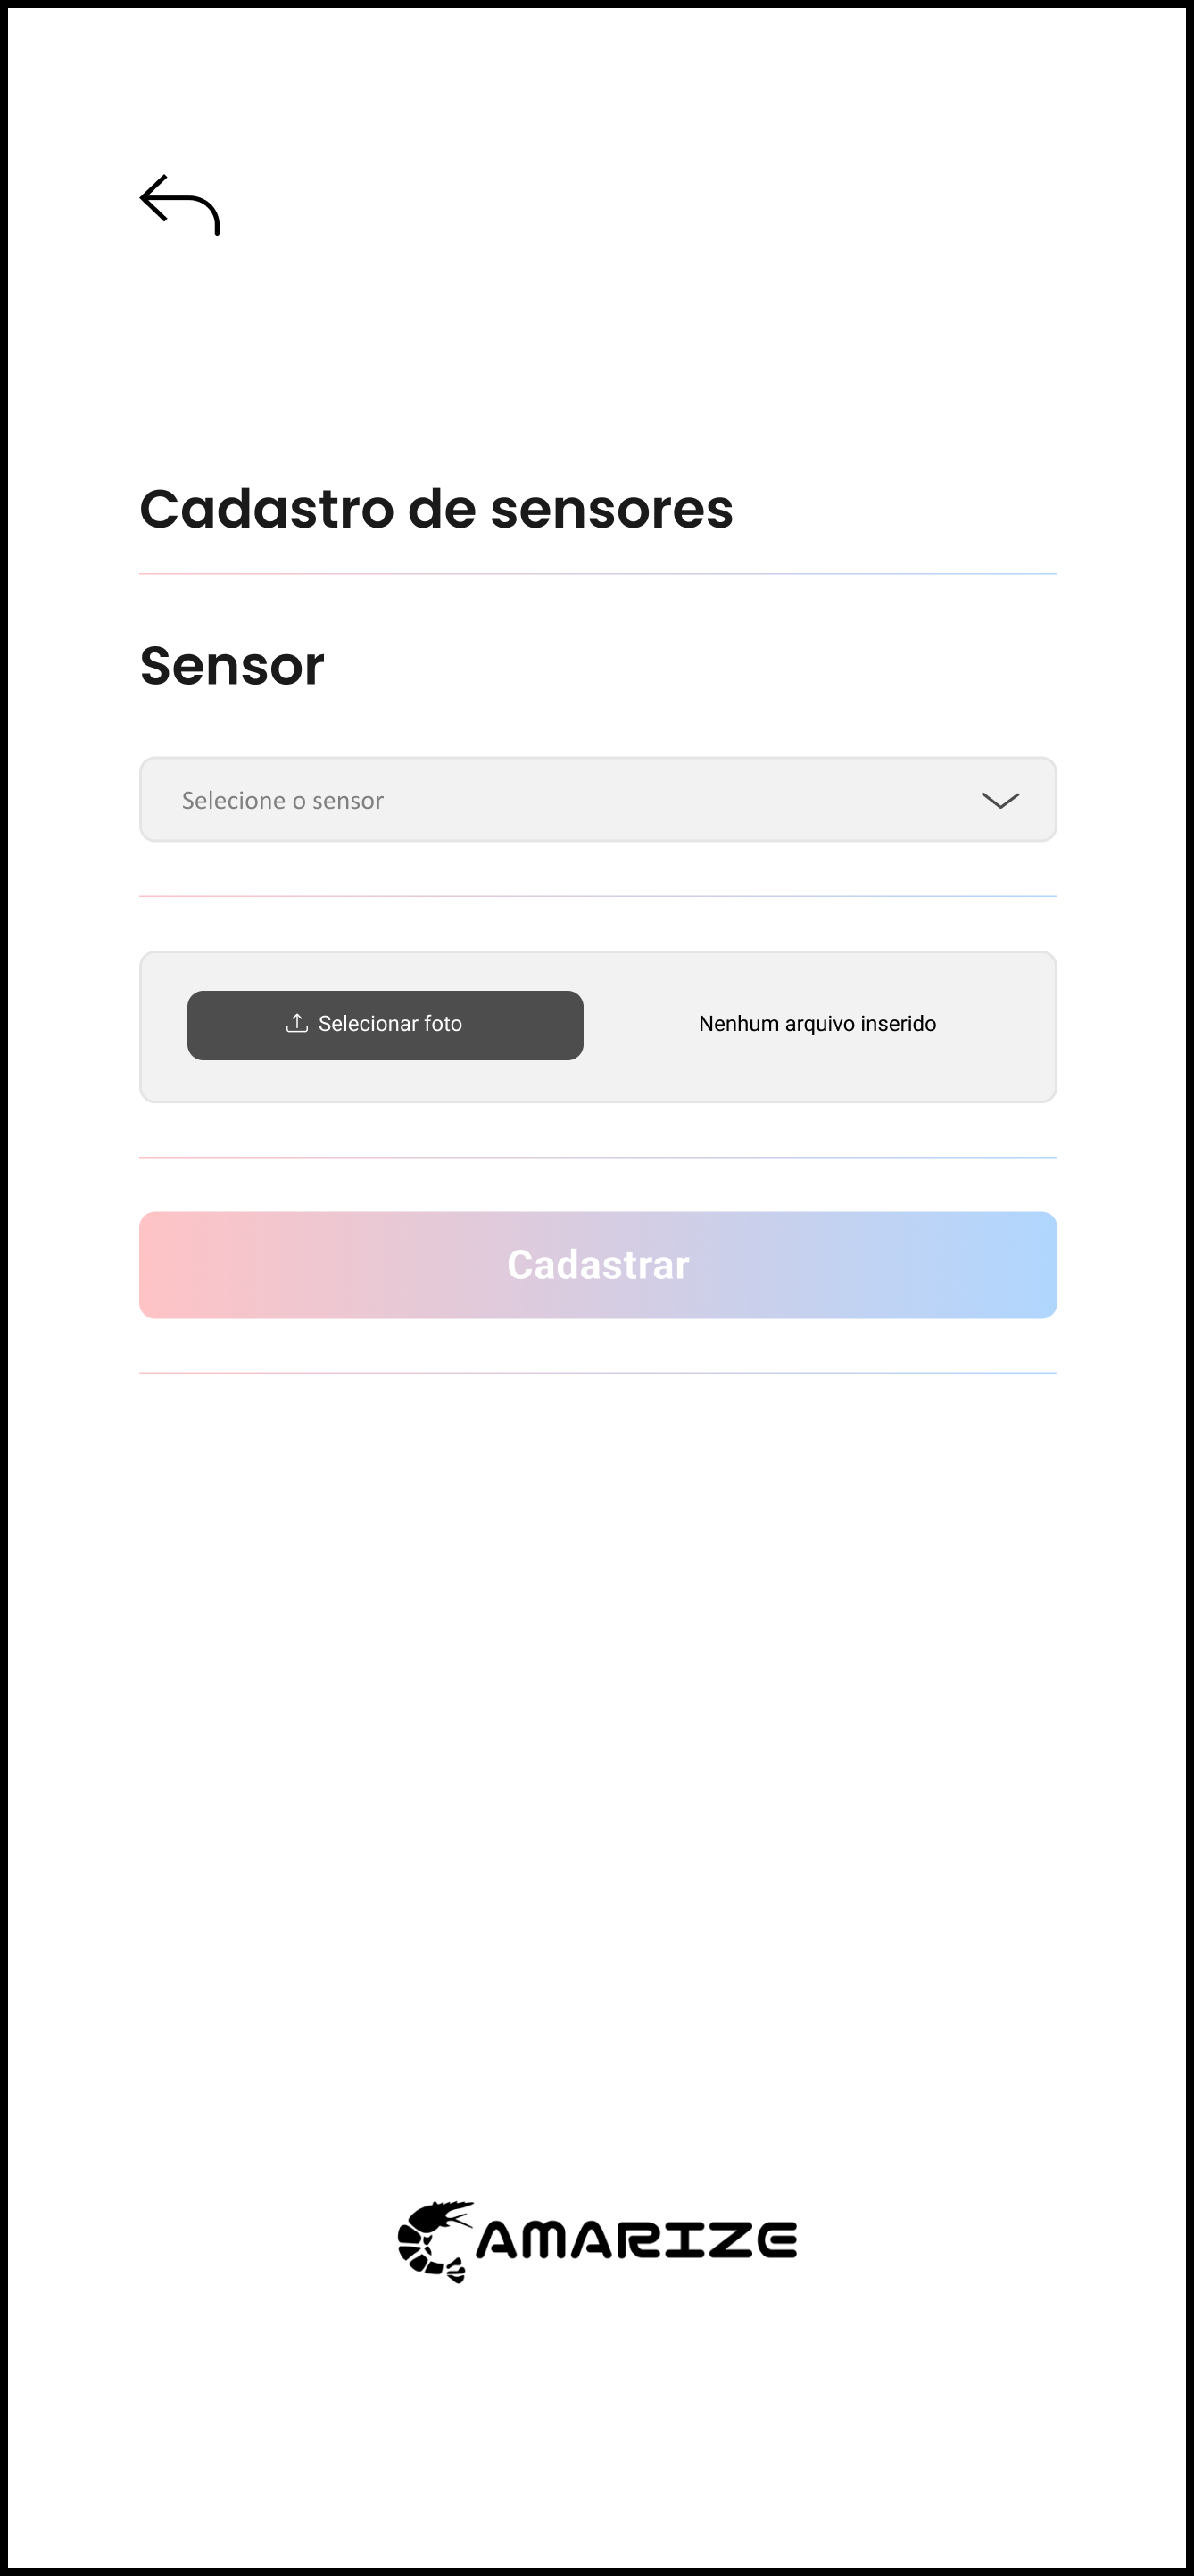
\includegraphics[width = 0.5\textwidth]{Imagem/Cadastrar_Sensor.png}
    \SourceOrNote{Autoria Própria, 2024}
\end{figure}

\newpage

Na Figura 6, é demonstrada a tela de cadastro de cada tanque, onde é selecionado o código de identificação do cativeiro, código de identificação do sítio e a data em que foi realizada a instalação do sistema.

\begin{figure}[!htb]
\centering
\SetCaptionWidth{\ifbool{@LayoutA}{0.7}{0.72}\linewidth}
\caption{Cadastro de Cativeiro}%
\label{fig:tela-cativeiro}
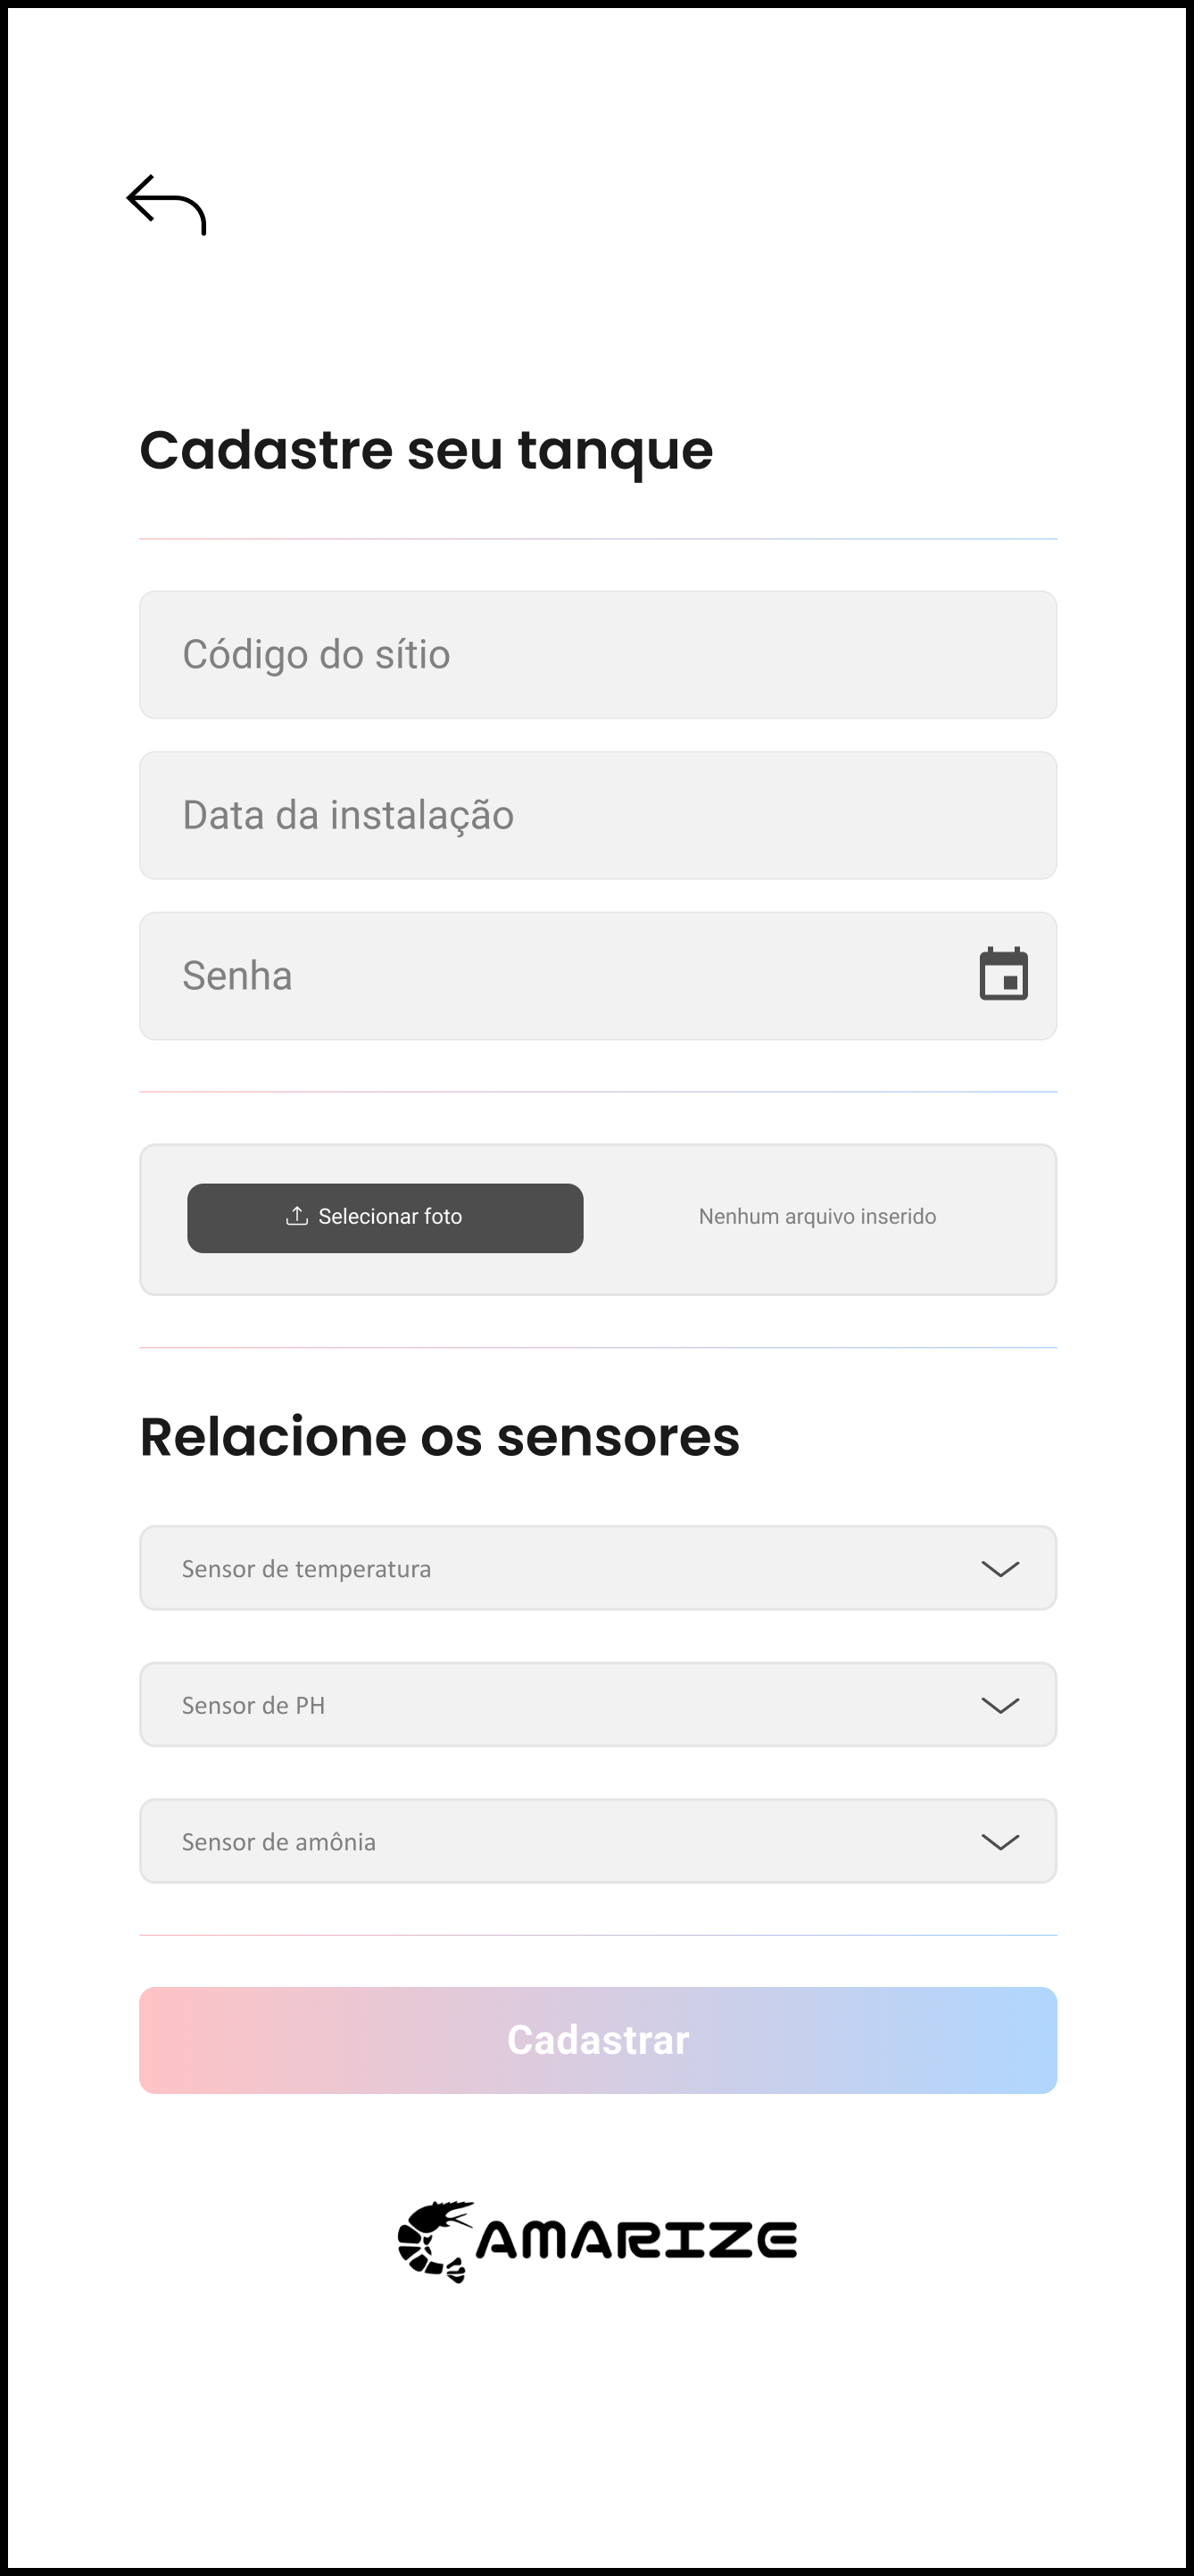
\includegraphics[width = 0.5\textwidth]{Imagem/Cadastrar_Cativeiro.png}
\SourceOrNote{Autoria Própria, 2024}
\end{figure}

\newpage

Na Figura 7, é apresentada a tela de notificações. O sistema irá notificar o usuário para caso ocorra algum tipo de mudança repentina em um dos cativeiros.

\begin{figure}[!htb]
    \centering
    \SetCaptionWidth{\ifbool{@LayoutA}{0.7}{0.72}\linewidth}
    \caption{Notificações}%
    \label{fig:notificações}
    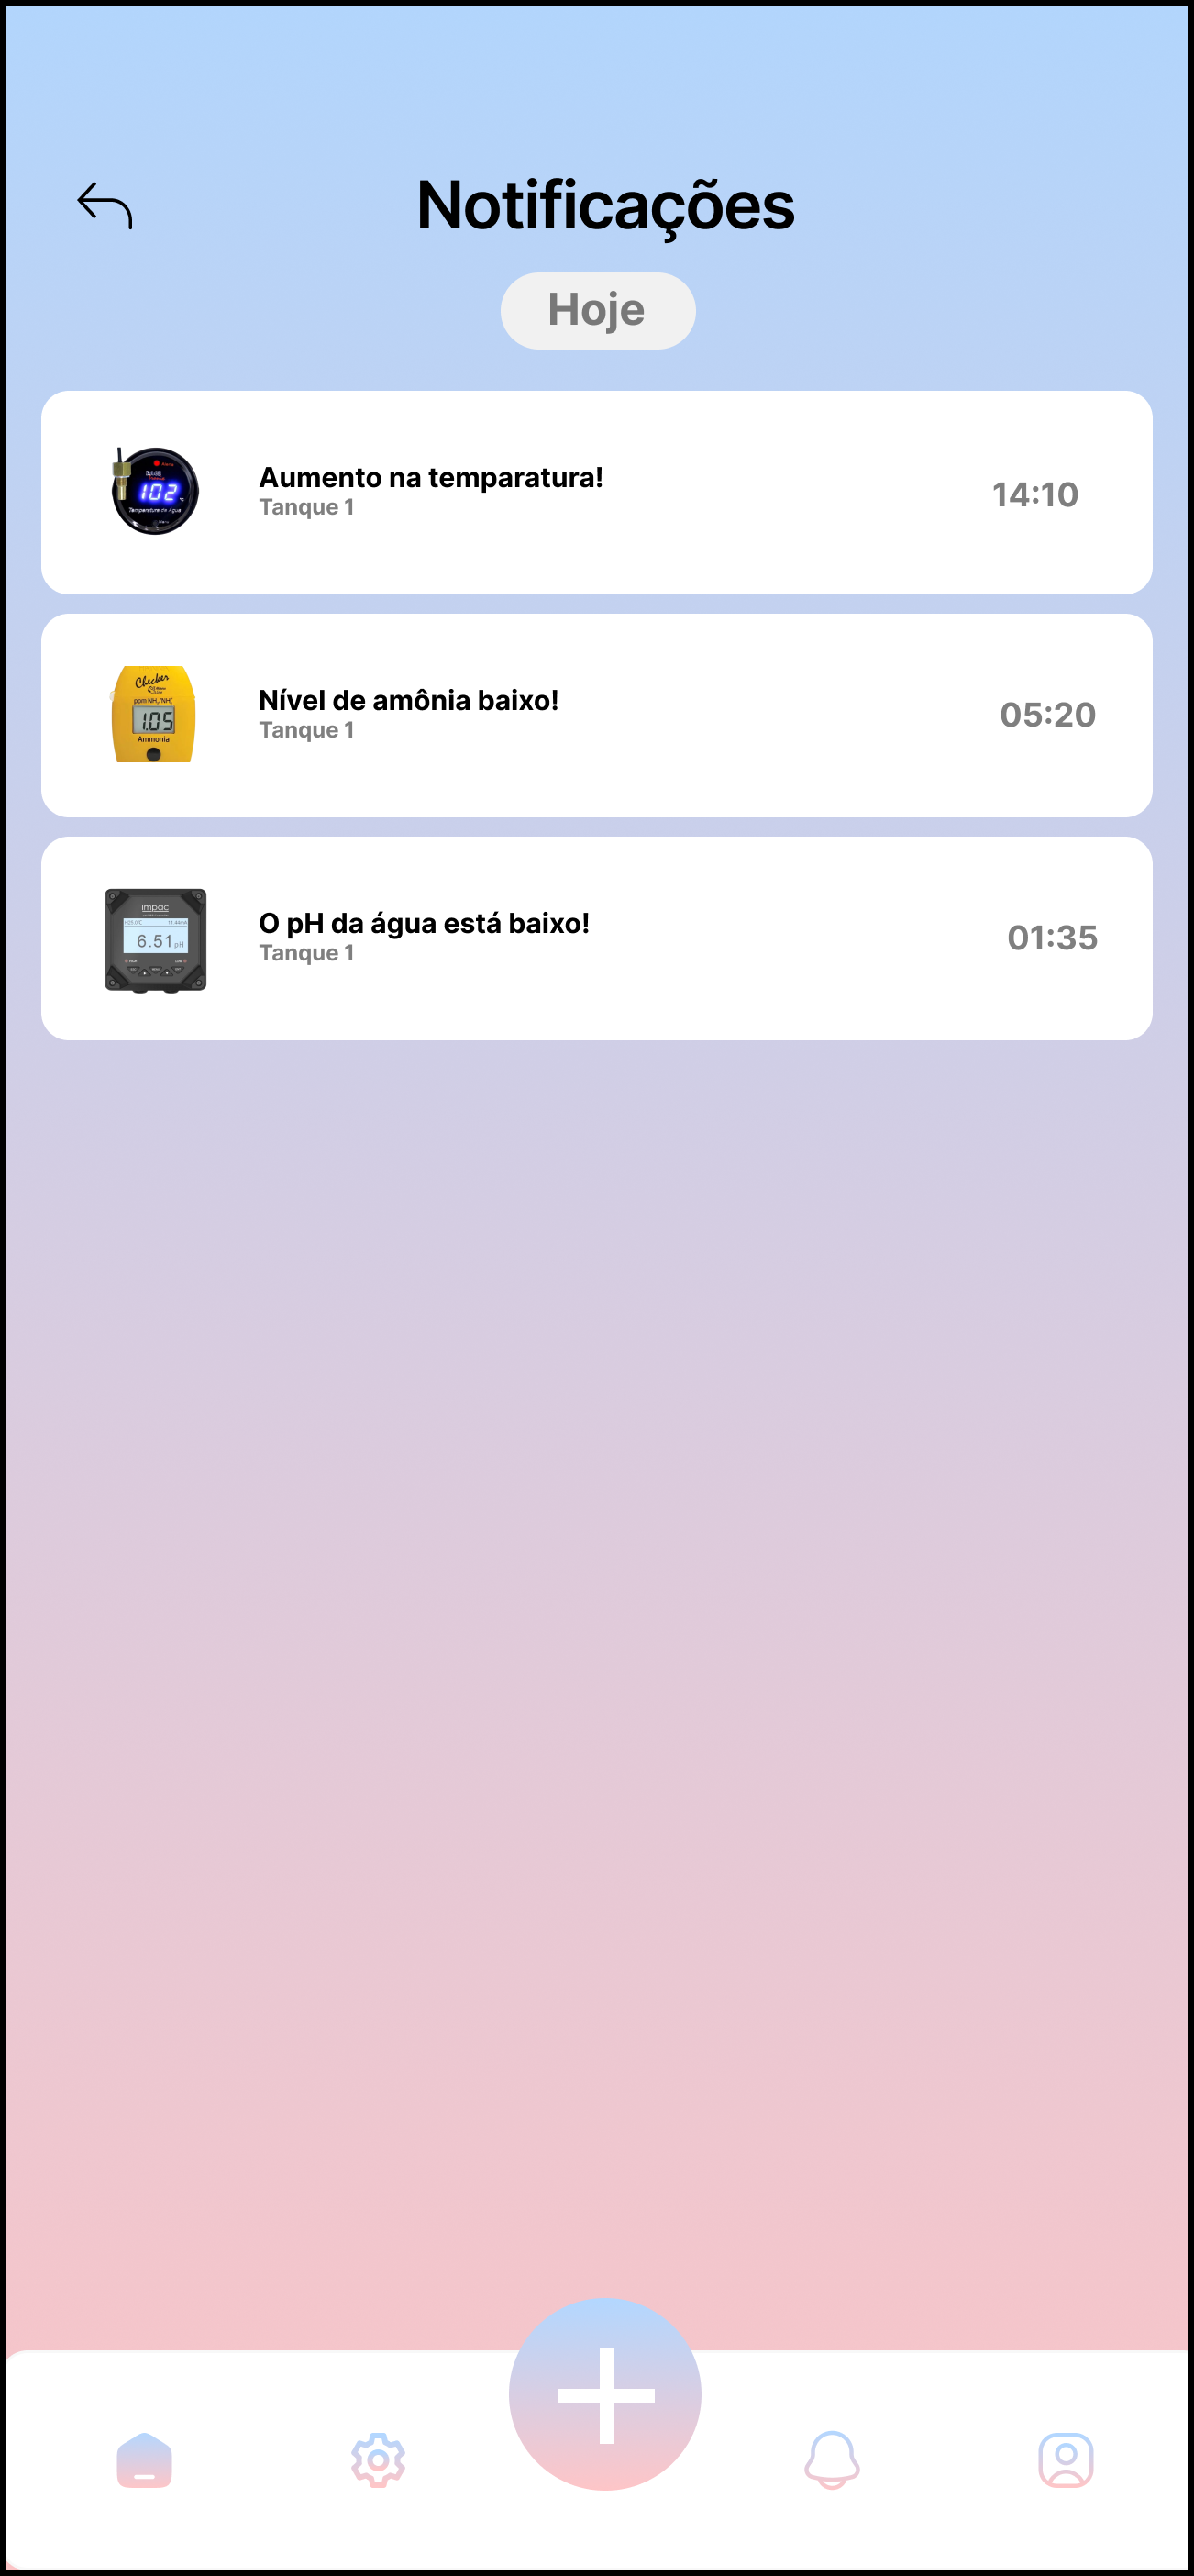
\includegraphics[width = 0.5\textwidth]{Imagem/Notificações.png}
    \SourceOrNote{Autoria Própria, 2024}
\end{figure}
    
\newpage

Na Figura 8, é demonstrada a tela de opções de relatório, onde é possível retirar relatórios sobre cada um dos tanques individualmente e de todos os tanques, sendo selecionado o período como semanal, mensal e anual.

\begin{figure}[!htb]
    \centering
    \SetCaptionWidth{\ifbool{@LayoutA}{0.7}{0.72}\linewidth}
    \caption{Relatórios}%
    \label{fig:relatório}
    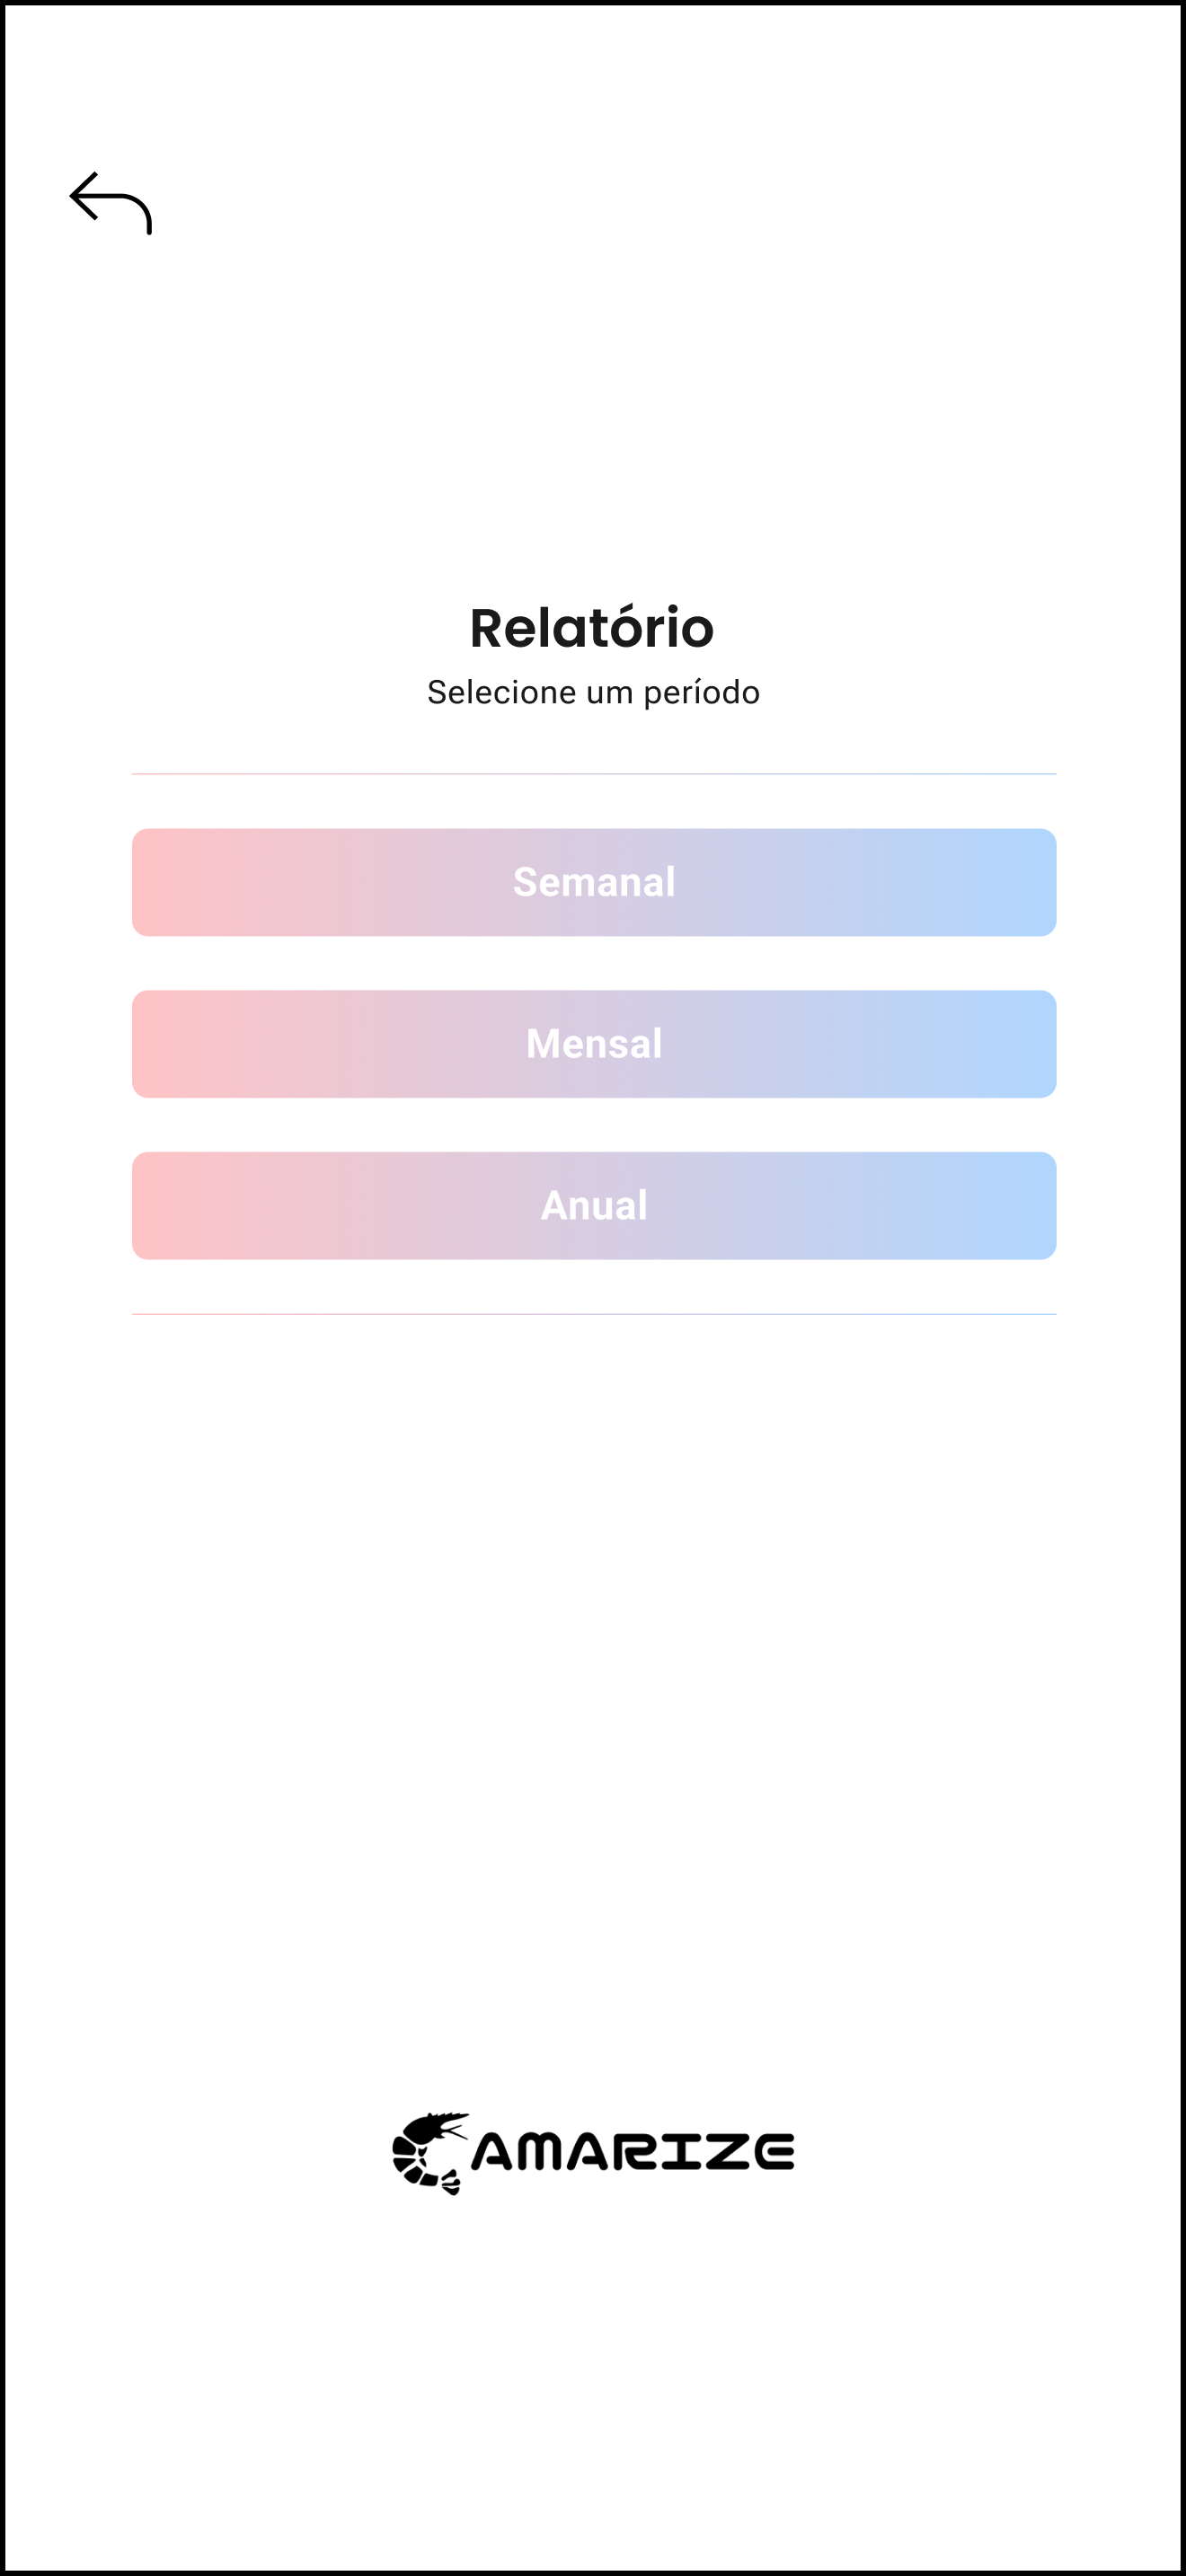
\includegraphics[width = 0.5\textwidth]{Imagem/Opções_Relatório.png}
    \SourceOrNote{Autoria Própria, 2024}
\end{figure}
    
\newpage

Na figura 9, apresenta um modelo de relatório, mostrando uma foto do cativeiro, o período selecionado e um resumo apresentando os dados e informações referentes ao tanque.

\begin{figure}[!htb]
    \centering
    \SetCaptionWidth{\ifbool{@LayoutA}{0.7}{0.72}\linewidth}
    \caption{Relatórios}%
    \label{fig:exemplo_relatório}
    \includegraphics[width = 0.5\textwidth]{Imagem/Relatório.png}
    \SourceOrNote{Autoria Própria, 2024}
\end{figure}
    
\newpage

\subparagraph*{\textbf{Desenvolvimento da aplicação}}

Por base nas telas mencionadas, foi realizado o desenvolvimento de nossa aplicação web. A aplicação foi desenvolvida por meio da linguagem JavaScript e a plataforma Node.js. A criação de um servidor HTTP se deu por meio da integração com o framework Express. Para realizar a renderização das telas HTML, foi feito uso do EJS (Embedded JavaScript).

Para armazenar as senhas de nossos usuários de maneira segura, foi utilizado a biblioteca ByCrypt. Essa bilbioteca fornece de um modo fácil e seguro o armazenamento de senhas utilizando um algoritmo denominado de Hash Forte e uma técnica chamada "Salting". Para cuidar da parte do banco de dados, se utilizou o Sequelize. O Sequelize permite a criação de modelos em JavaScript que representam o banco de dados, podendo assim manipular os dados utilizando objetos e métodos.

Para gerenciar as sessões dos usuários e integração de métodos de autenticação, foi utilizado o middleware Express-Session, que armazena os dados da sessão no servidor.

Com o objetivo de manter a organização do código, foi feito uso do modelo de arquitetura MVC (Model, View, Control). Model é resposnável por lidar com os dados e regras impostas na aplicação, View é responsável por lidar com a interação com usuários e os dados que são fornecidos, Control atua como um intermediário entre Model e View, processando as solicitações e manipulação de dados.

Para facilitar a navegação do usuário, foram implementadas rotas. As rotas cuidam dos pontos de acesso da aplicação, mapeando as requisições HTTP para determinadas funções, permitindo com que o usuário interaja com cada parte desenvolvida na aplicação.

\subparagraph*{\textbf{Diagrama de Caso de Uso}}

Com o Diagrama de Caso de Uso (DCU) apresentada na figura 10, é possível verificar as interações entre o usuário, visto como o carcinicultor, e o sistema. Essas interações incluem desde a realização da conta até a analise completa de cada funcionalidade do sistema, como relatório geral, visualização dos tanques e utilização do modo automático de alimentação.

\begin{figure}[!htb]
\centering
\SetCaptionWidth{\ifbool{@LayoutA}{0.7}{0.72}\linewidth}%
\caption{Diagrama de Caso de Uso}%
\label{fig:caso-uso}
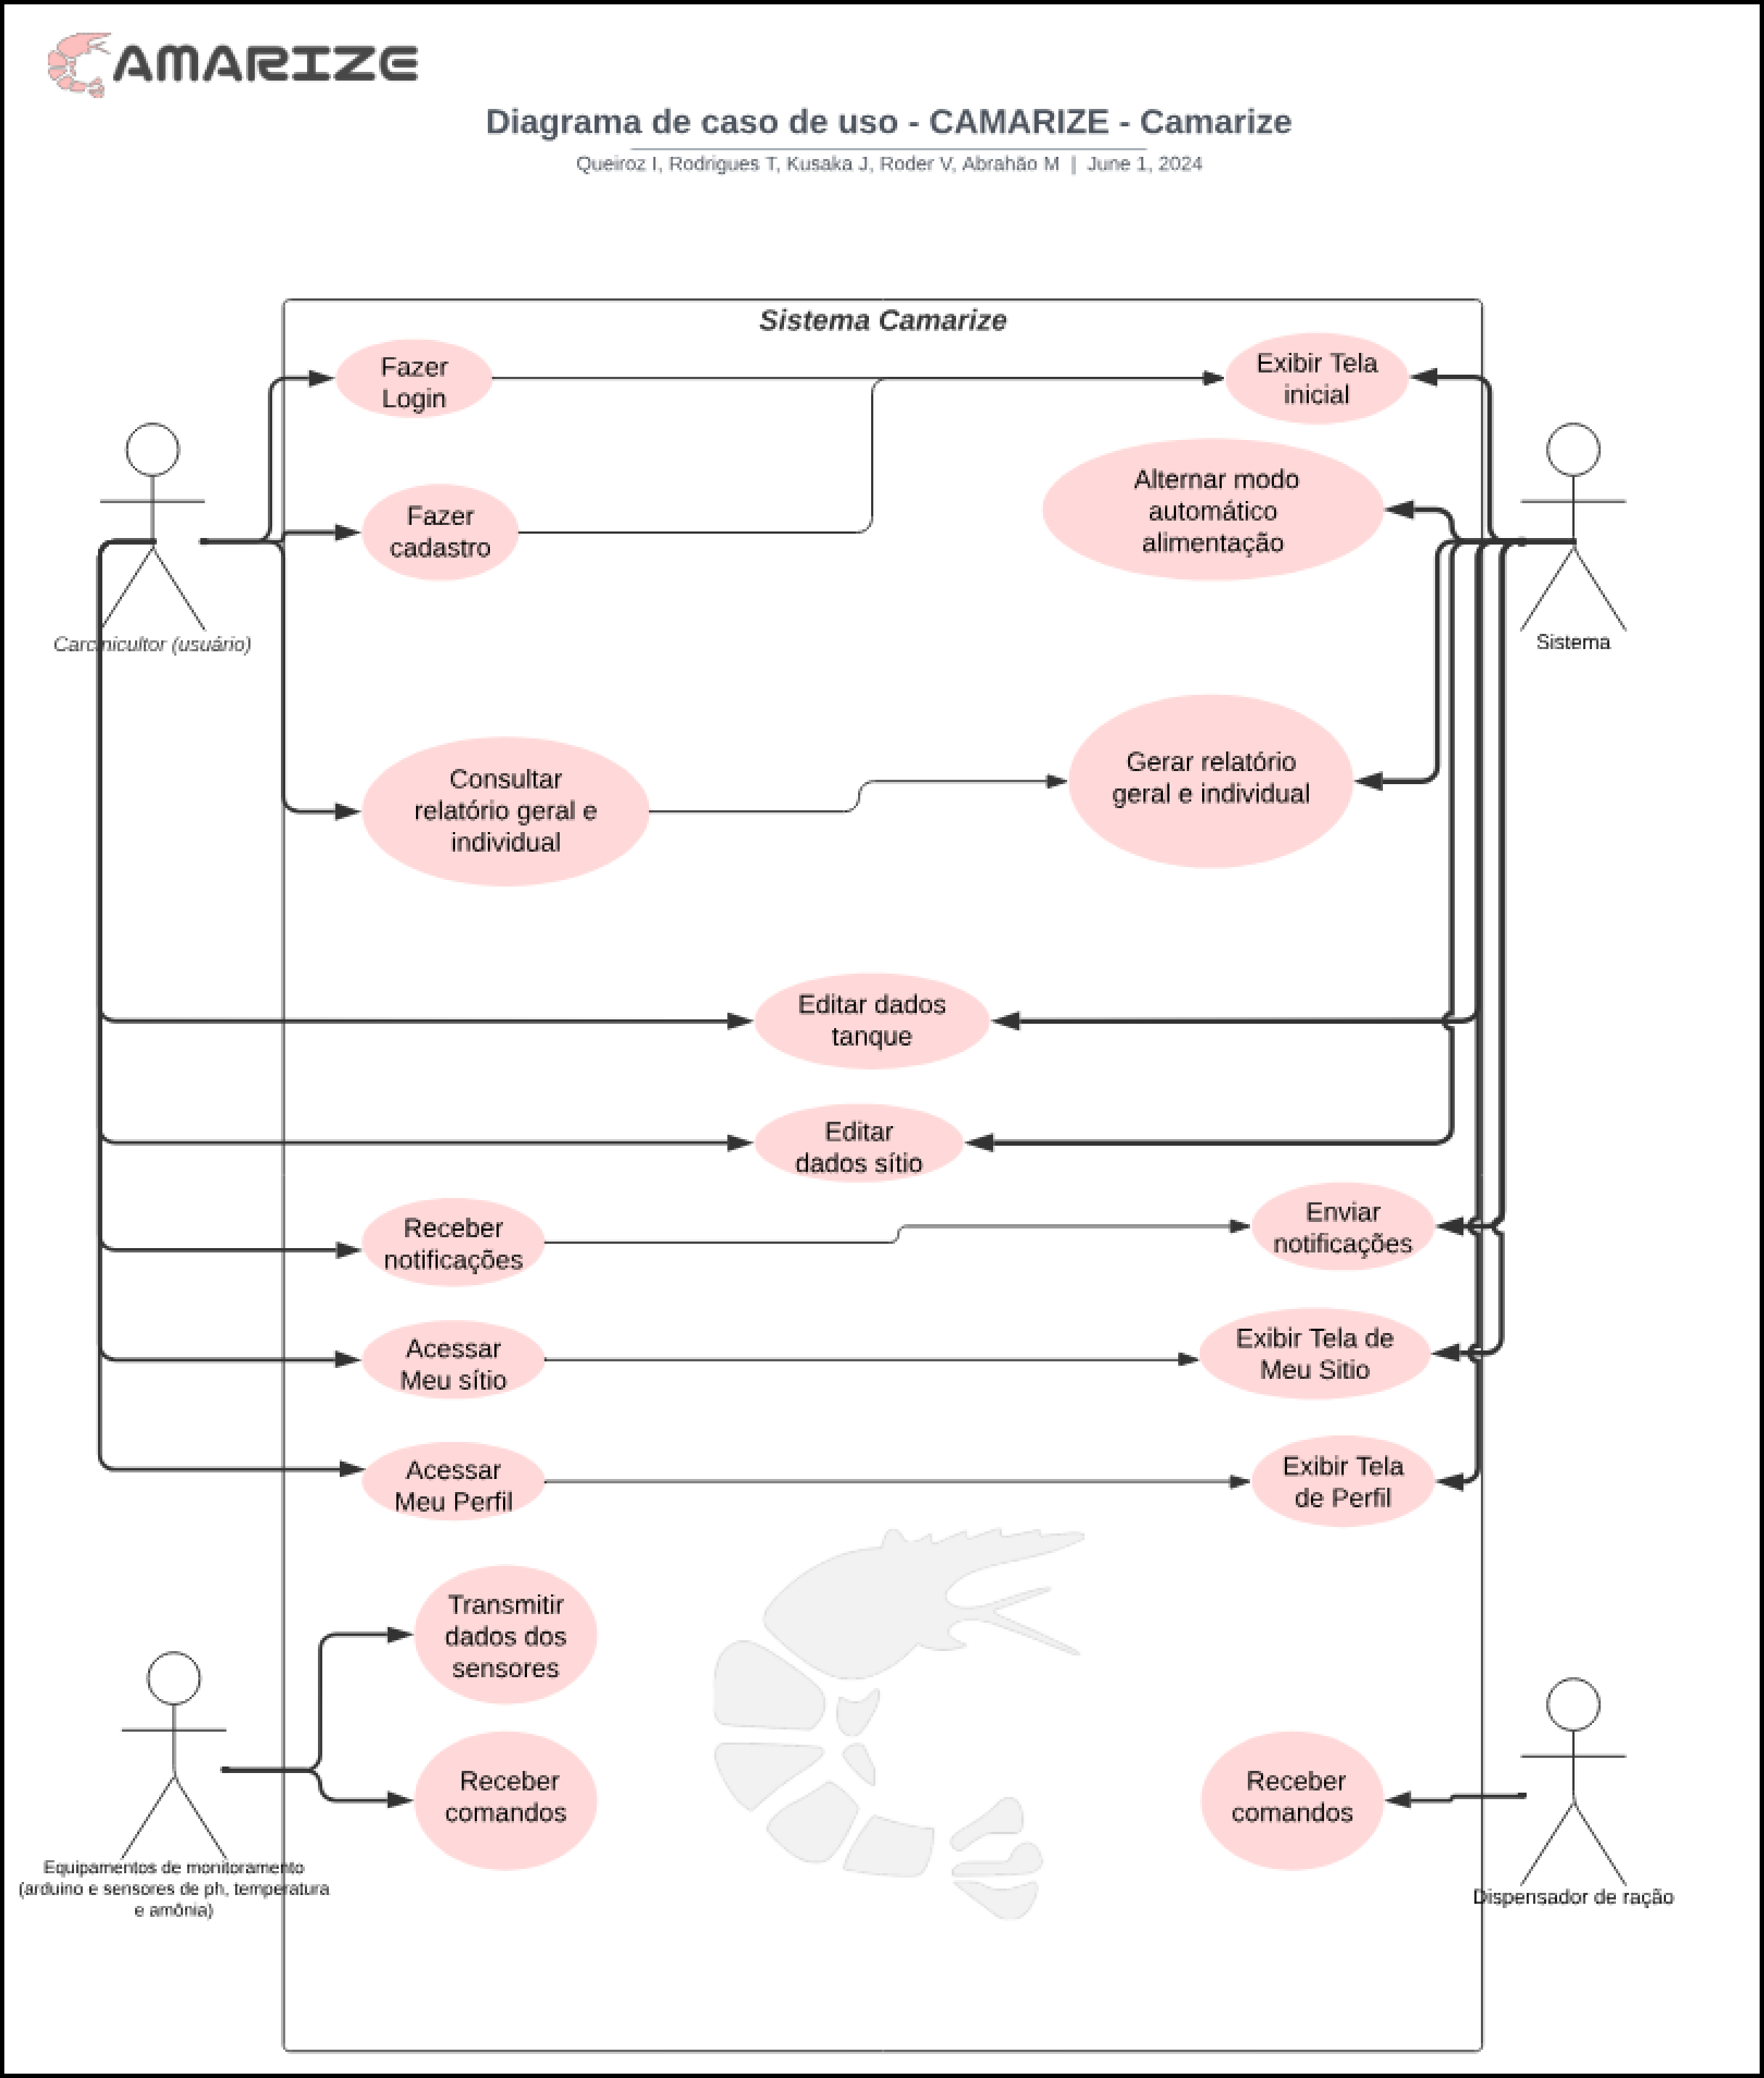
\includegraphics[width = 1.3\CaptionWidth]{Imagem/Caso de Uso.png}
\SourceOrNote{Autoria Própria, 2024}
\end{figure}

\newpage

\subparagraph*{\textbf{Diagrama de Classe}}

Com o Diagrama de classe na figura 11, pode-se ter noção das funcionalidades e atributos que estão presentes dentro do sistema, partindo de funcionalidades simples até mais complexas, podendo entender suas ligações entre cada uma das classes.    

    \begin{figure}[!htb]
        \centering
        \SetCaptionWidth{\ifbool{@LayoutA}{0.7}{0.72}\linewidth}%
        \caption{Diagrama de Classe}%
        \label{fig:classe}
        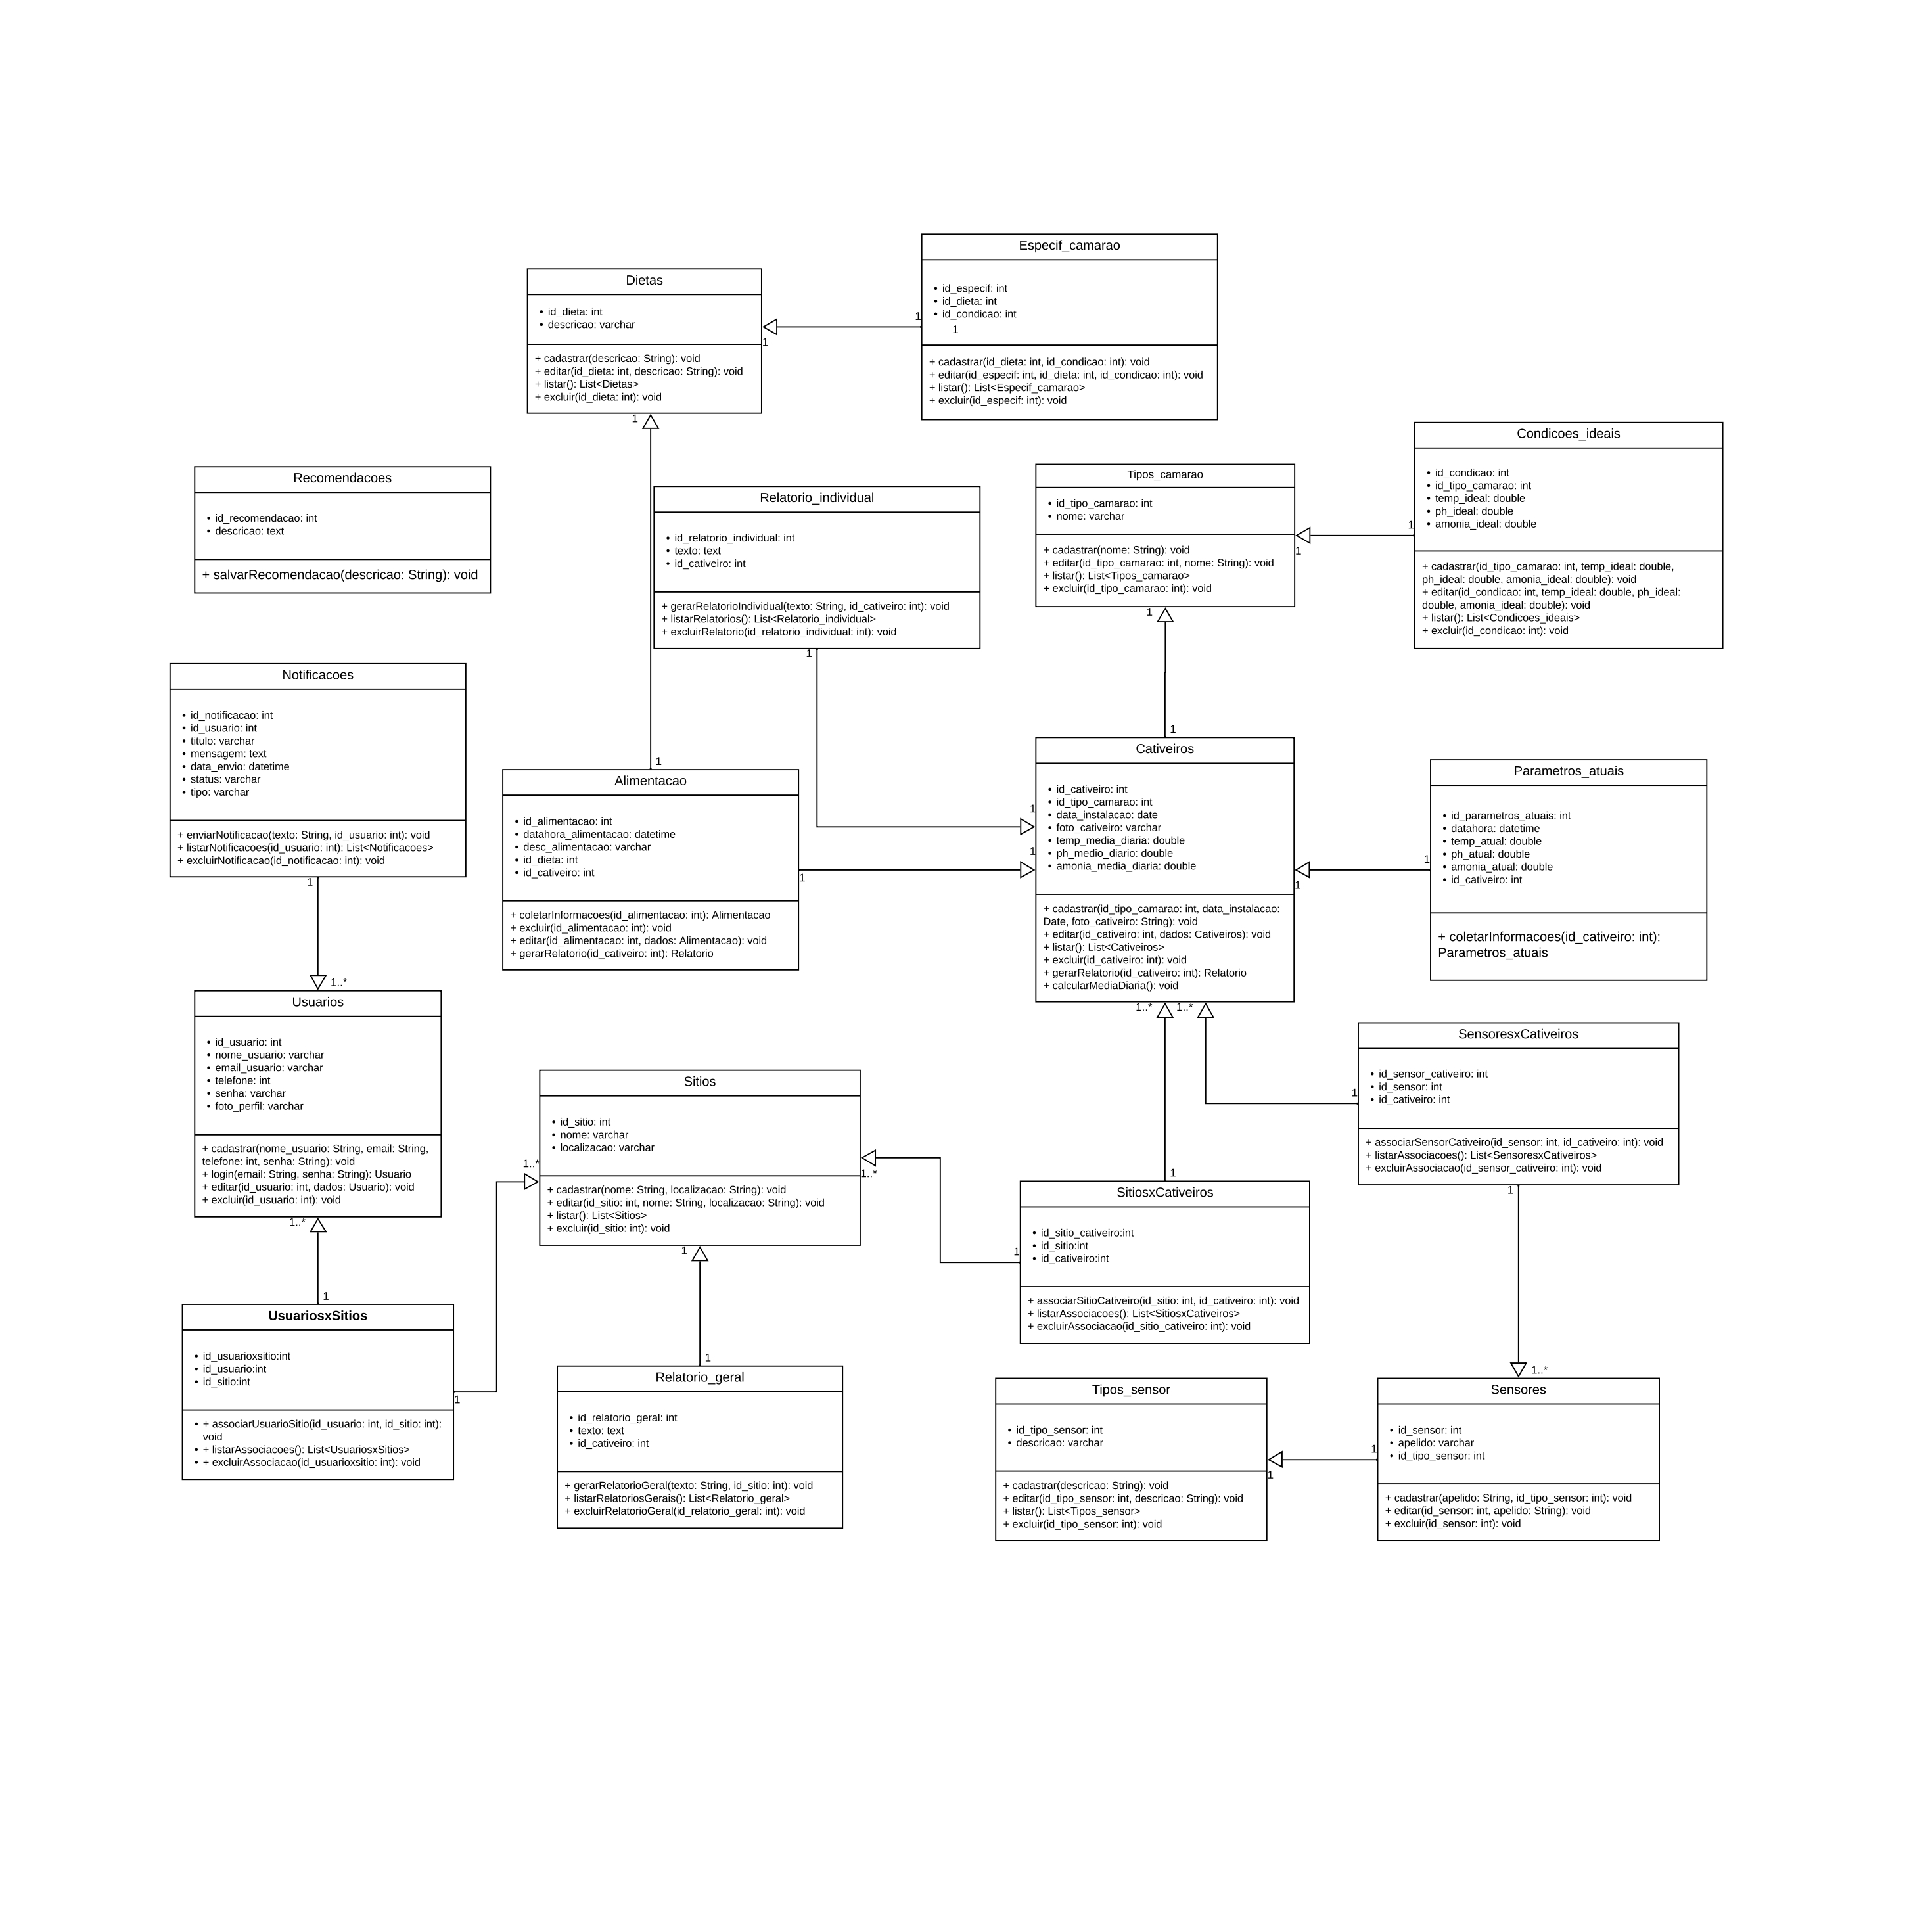
\includegraphics[width = 1.6\CaptionWidth]{Imagem/Diagramas de Classe.jpg}
        \SourceOrNote{Autoria Própria, 2024}
    \end{figure}

\newpage

\subparagraph*{\textbf{Diagrama de Objetos}}

Com base no Diagrama de objetos na figura 12, é possível visualizar situações específicas do sistema, apresentando situações específicas do sistema, mostrando como os objetos se interagem e colaboram em uma situação real.

\begin{figure}[!htb]
    \centering
    \SetCaptionWidth{\ifbool{@LayoutA}{0.7}{0.72}\linewidth}%
    \caption{Diagrama de Objetos}%
    \label{fig:objetos}
    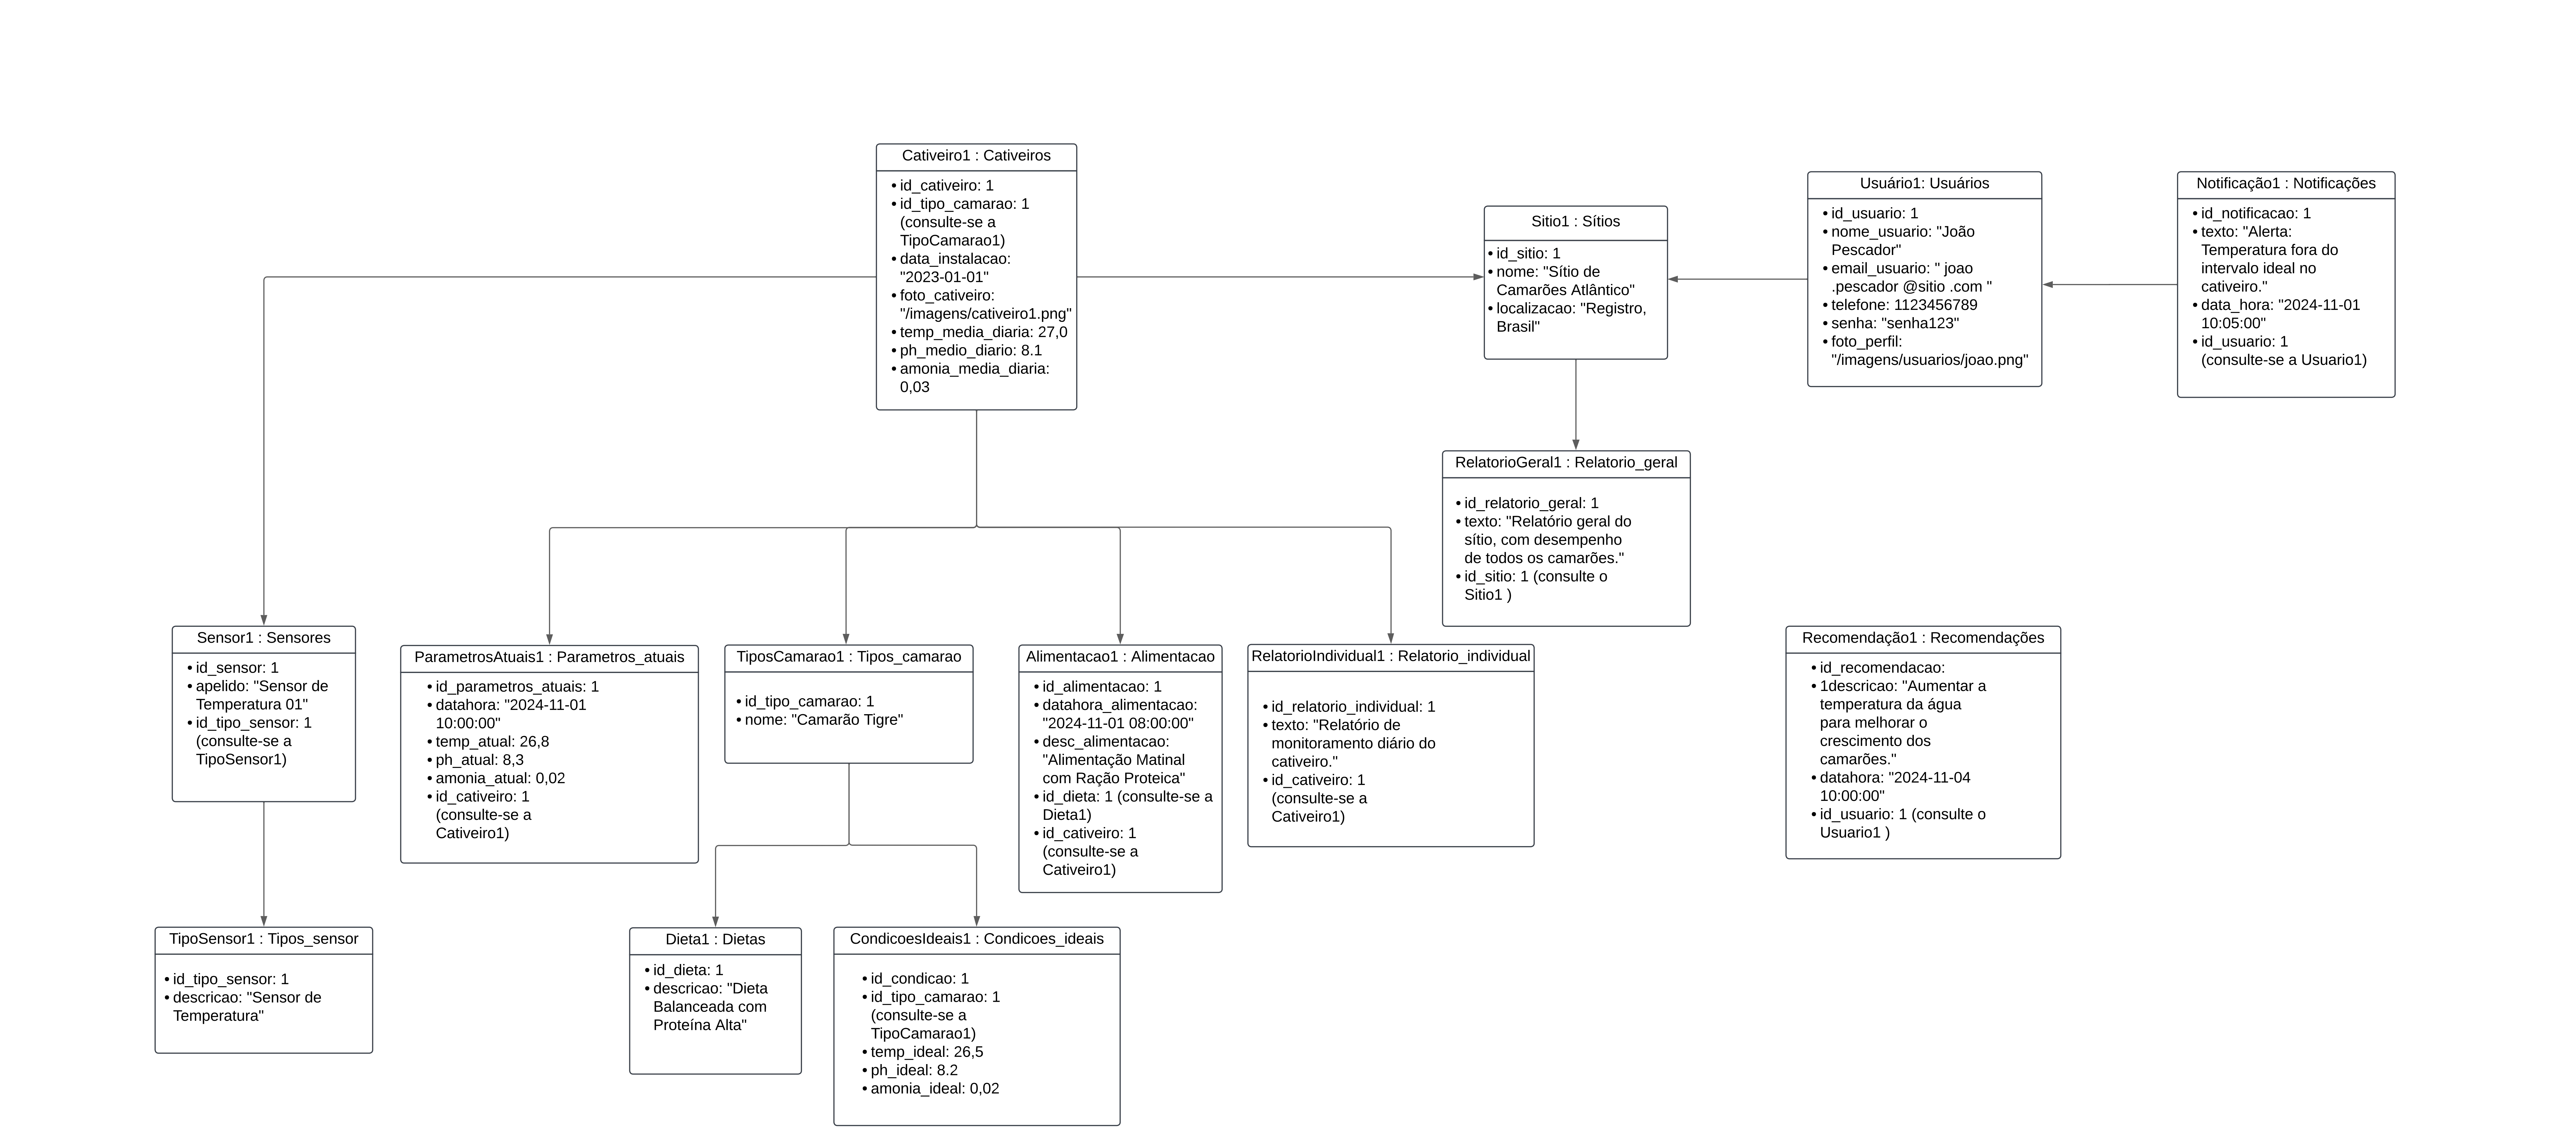
\includegraphics[width = 1.6\CaptionWidth]{Imagem/Diagrama de Objetos.jpg}
    \SourceOrNote{Autoria Própria, 2024}
\end{figure}

\newpage


\subparagraph*{\textbf{Modelagem Lógica, Conceitual e Física do Banco de Dados}}

O banco de dados tem um papel de extrema importância para as informações, sendo necessário para guardar, organizar e recuperar dados. O Modelo Lógico e Conceitual são maneira de demonstrar a eficiência de um banco de dados.

A modelagem conceitual, lógica e física, representadas na Figura 13, Figura 14 e Figura 15, demonstram a funcionalidade do programa e do que será aplicado no banco de dados. A visão gráfica do banco de dados se demonstra algo fundamental, por conta que proporciona o máximo de detalhes com extrema clareza, apresentando as relações entre as entidades.

No modelo conceitual, Camarões está ligado com Cativeiro por meio de Tipos de Camarões, apresentando característica como espécie e peso. Com os Cativeiros fazendo parte de Sítios, pode-se realizar o Monitoramento por meio de Sensores e controlar a Alimentação dos camarões. O Monitoramento possui Temperatura, pH e Amônia fazendo assim o registro de cada um. Alimentação possui o horário que foi realizado a alimentação e a quantidade de alimento fornecida para cada Cativeiro.

No modelo lógico, é apresentado uma representação mais concreta do banco de dados, demonstrando as tabelas, entidades, chaves primárias e estrangeiras e seus relacionamentos.

No modelo físico, demonstra uma versão refinada do modelo conceitual, representando restrições de dados, nomes de entidades e relacionamentos para implementação de forma independente.

    \newpage

    \begin{figure}[!htb]
    \SetCaptionWidth{\ifbool{@LayoutA}{0.7}{0.72}\linewidth}
    \caption{Modelo Conceitual}%
    \label{fig:conceitual}
    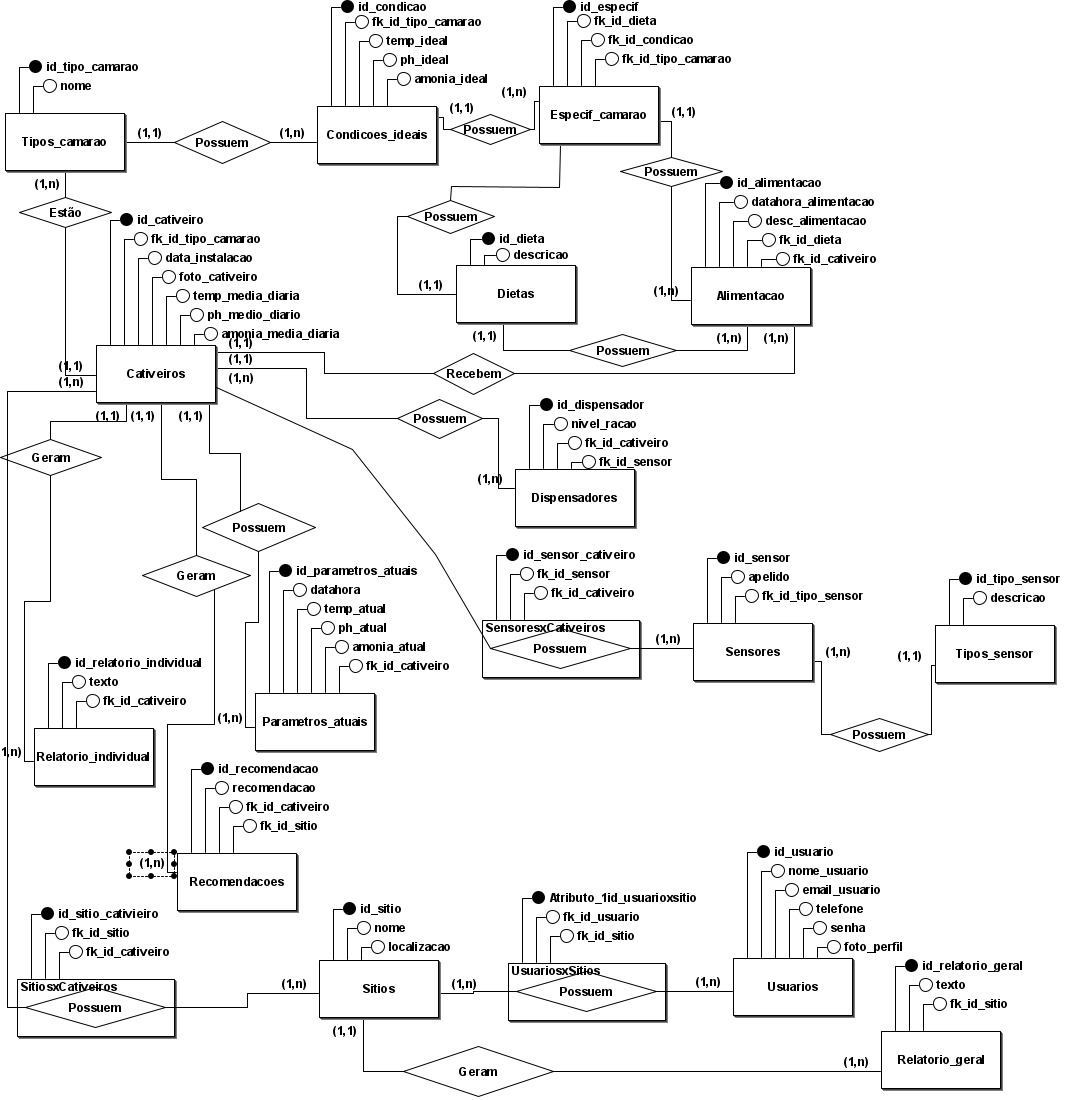
\includegraphics[width = 1\CaptionWidth]{Imagem/Modelo Conceitual.jpeg}
    \SourceOrNote{Autoria Própria, 2024}
    \end{figure}

    \newpage

    \begin{figure}[!htb]
    \SetCaptionWidth{\ifbool{@LayoutA}{0.7}{0.72}\linewidth}
    \caption{Modelo Lógico}%
    \label{fig:logico}
    \includegraphics[width = 1.3\CaptionWidth]{Imagem/Modelo Lógico.png}
    \SourceOrNote{Autoria Própria, 2024}
    \end{figure}

    \newpage

    \begin{figure}[!htb]
    \SetCaptionWidth{\ifbool{@LayoutA}{0.7}{0.72}\linewidth}
    \caption{Modelo Físico}%
    \label{fig:fisico}
    \includegraphics[width = 1.3\CaptionWidth]{Imagem/Modelo Físico.jpg}
    \SourceOrNote{Autoria Própria, 2024}
    \end{figure}

\subparagraph*{\textbf{Modelo de Negócio Canvas}}

O modelo de negócios Canvas foi utilizado para análise econômica do sistema. Por meio do Canvas foi possível identificar os Parceiros, Recursos e Atividades Chaves, nossas Propostas de Valor, Segmento de Mercado, nossa Fonte de Renda e Estrutura de Custos.

\newpage

    \begin{figure}[!htb]
        \centering
        \SetCaptionWidth{\ifbool{@LayoutA}{0.7}{0.72}\linewidth}
        \caption{Canvas}%
        \label{fig:canvas}
        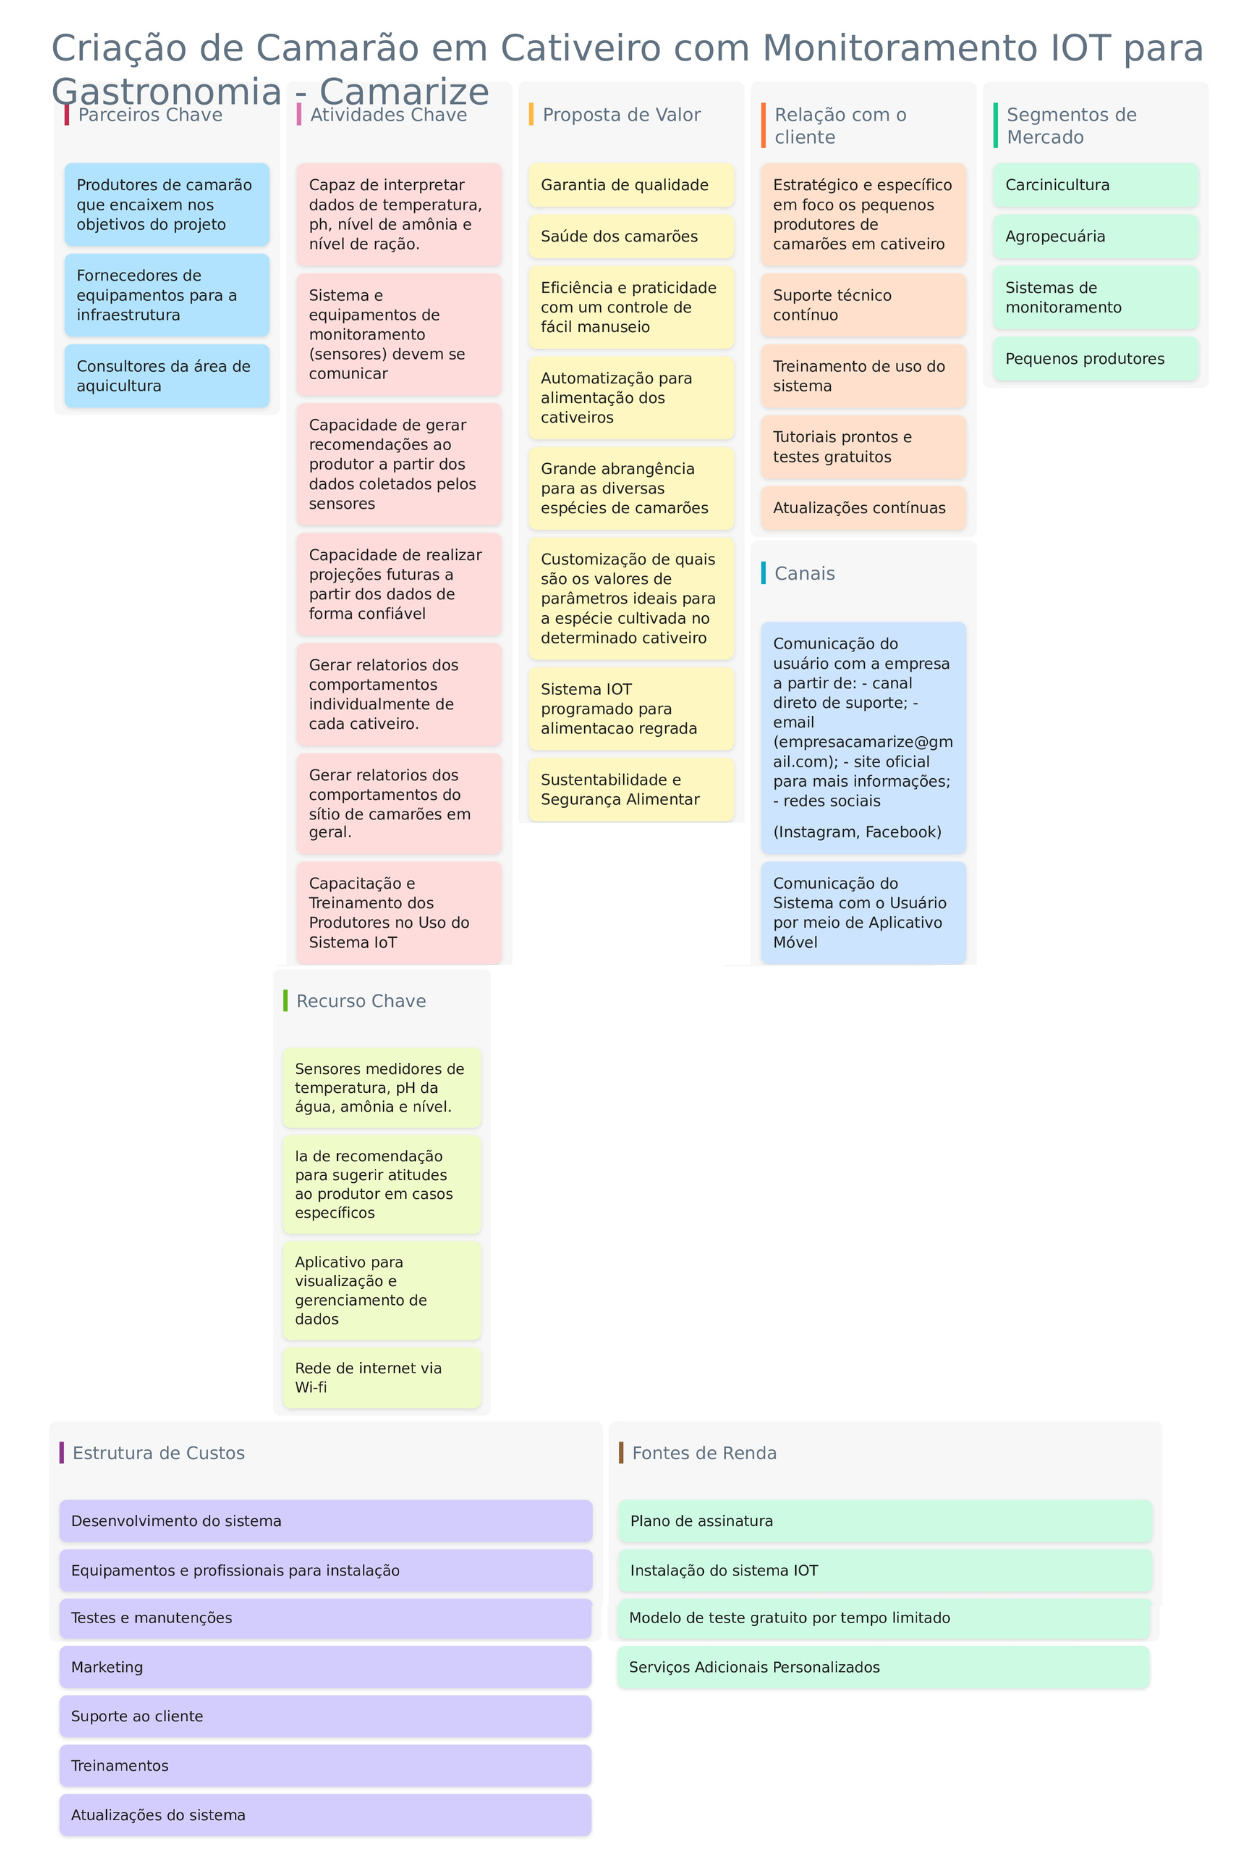
\includegraphics[width = 1.1\CaptionWidth]{Imagem/Canvas.png}
        \SourceOrNote{Autoria Própria, 2024}
    \end{figure}

\newpage

\subparagraph*{\textbf{Análise de recorrência do algoritmo Merge Sort}}

O Merge Sort é um algoritmo de ordenação que consiste em dividir uma estrutura de subconjuntos e aplicar a ordenação nos elementos que são extraídos da estrutura primária. Após a ordenação dos subconjuntos, é realizada a mistura para um conjunto final ordenado.

O melhor tempo ocorre quando todos os elementos do array já estão ordenados, o Merge Sort sempre executa a divisão e a fusão, independente  da ordem dos elementos. O tempo de execução, representado por \( O(n \log_2 n) \), pode ser explicado da seguinte forma: \( \log_2 n \) corresponde ao número de divisões do array até que cada subarray contenha apenas um elemento, e \( n \) refere-se ao número de comparações e fusões realizadas durante o processo de merge.

O tempo médio ocorre quando os elementos estão em ordens aleatórias, em seu comportamento o número de divisões e fusões não dependem da ordem dos elementos, cada nível realiza \( n \) operações no total e possui \( \log_2 n \) níveis. Sua representação é semelhante com o melhor tempo: \( O(n \log_2 n) \).

O pior tempo ocorre quando o array está em ordem oposta a esperada, sua complexidade não é alterada por conta que sua quantidade de execuções não são alteradas. Sua representação se mantém a mesma, sendo ela: \( \log_2 n \).

Na aplicação, foi utilizada na tela de sensores, sendo utilizado para organizar os sensores de forma crescente e decrescente. Seu tempo de execução foram exatos 0.000000 milisegundos, mostrando a eficiência e rapidez do algoritmo. Sua representação matemática se apresenta desta maneira:

\[
\text{MergeSort}(n) =
\begin{cases}
0, & \text{se } n = 0 \\
0, & \text{se } n = 1 \\
2 \cdot \text{MergeSort}\left(\frac{n}{2}\right) + O(n), & \text{se } n > 1
\end{cases}
\]


\textbf {A representação em pseudocódigo:} 


\begin{verbatim}
    funcao mergeSort(arr[])

    // Função recursiva para ordenar o vetor usando o algoritmo MergeSort

    se tamanho de arr <= 1 então
        retornar arr
    fimse

    meio <- arredondar_para_baixo(arr.length / 2)
    esquerda <- mergeSort(arr[0, meio])
    direita <- mergeSort(arr[meio, arr.length])

    retornar merge(esquerda, direita)
fimfuncao

funcao merge(esquerda[], direita[])

    // Função para combinar dois vetores ordenados

    resultado <- lista_vazia
    indice_esquerda <- 0
    indice_direita <- 0

    enquanto indice_esquerda < tamanho de esquerda e 
    indice_direita < tamanho de direita faça
    se 
    esquerda[indice_esquerda].id_tipo_sensor > direita[indice_direita].id_tipo_sensor 
        então
            adicionar esquerda[indice_esquerda] em resultado
            indice_esquerda incrementa 1
        senão
            adicionar direita[indice_direita] em resultado
            indice_direita incrementa 1
        fimse
    fimenquanto

    retornar resultado concatenado com esquerda[indice_esquerda, arr.length] 
    e direita[indice_direita, arr.length]
fimfuncao
    \end{verbatim}
